\documentclass[runningheads, 11pt]{llncs}
%\documentclass{amsart}
\usepackage{epsfig}
%\usepackage{epic}
\usepackage{latexsym}
\usepackage{amsmath}
%\setlength{\unitlength}{1mm}
%\parskip=1em


%\usepackage[ruled]{algorithm2e}
\usepackage{graphicx}
\usepackage{amsmath}
\usepackage{amssymb}
%\usepackage{ulem}
\usepackage[normalem]{ulem} 
\usepackage{cancel}

\setlength{\textwidth}{6.4in}
\setlength{\textheight}{9.4in}
\setlength{\topmargin}{-0.6in}
\setlength{\oddsidemargin}{0in}
\setlength{\evensidemargin}{0in}
%\setlength{\headsep}{.3in}

\newtheorem{thm}{Theorem}
%\newtheorem{lemma}[thm]{Lemma}
%\newtheorem{problem}[thm]{Problem}
\newtheorem{prop}[thm]{Proposition}
\newtheorem{cor}[thm]{Corollary}
%\theoremstyle{definition}
\newtheorem{defn}[thm]{Definition}
%\newtheorem{example}[thm]{Example}
%\newtheorem{remark}[thm]{Remark}
\newtheorem{conj}[thm]{Conjecture}
\newtheorem{observation}[thm]{Observation}

\newcommand{\cherry}[1]{\ensuremath{\langle #1 \rangle}}
\newcommand{\ignore}[1]{}
\newcommand{\half}{\frac{1}{2}}
\newcommand{\eopf}{\framebox[6.5pt]{} \vspace{0.2in}}
\newcommand{\cE}{\mathcal{E}}
\newcommand{\MM}{\mathcal{M}}
\newcommand{\EE}{\mathbb{E}}
\newcommand{\PP}{\mathbb{P}}
\newcommand{\R}{\mathcal{R}}
\newcommand{\Q}{\mathcal{Q}}
\newcommand{\A}{\mathcal{A}}
\newcommand{\cH}{\mathcal{H}}
\newcommand{\cP}{\mathcal{P}}
\newcommand{\G}{\mathcal{G}^{(n)}}
\newcommand{\Neigh}[2]{N_{2k}\left ( #1,\mathcal{G}^{(n)}( #2 ) \right )}
\usepackage{color}
\usepackage{hyperref}

\newcommand{\Red}[1]{{\color{red}#1}}


%------------------document begins-----------------------

\title{Sorting the Deep Branches of the Prokaryotic Tree: A First Statistical
Approach}

\author{Gur Sevillya\thanks{Department of Evolutionary and Environmental
Biology, University of Haifa, Israel,} \and 
Yael Lerner \thanks{Department of Evolutionary and Environmental Biology,
University of Haifa, Israel,} \and 
Daniel Doerr\thanks{ Faculty of Technology, Bielefeld University, Germany, }
\and
Jens Stoye\thanks{ Faculty of Technology, Bielefeld University, Germany, } \and
Sagi Snir$^{a}$\thanks{Department of Evolutionary and Environmental Biology,
University of Haifa, Israel,} \and 
Mike Steel\thanks{School of Mathematics and Statistics, University of
Canterbury, NZ.}}
\institute{University of Haifa}

\date{ }

\begin{document}
%\noindent \maketitle

\begin{center}
\noindent{\Large \bf Horizontal Gene Transfer Phylogenetics: A First
Model-Based Approach}
\end{center}
\bigskip
\noindent {\normalsize \sc Gur Sevillya$^1$, Yael Lerner$^1$,
 Daniel Doerr$^2$, Jens Stoye$^2$, Mike Steel$^{3,*}$, and Sagi Snir$^{1,*}$ }\\
\noindent {\small \it 
$^1$Dept. of Evolutionary Biology, University of Haifa, Israel\\
\noindent
$^2$Faculty of Technology, Bielefeld University, Germany\\
\noindent
$^3${School of Mathematics and Statistics, University of
 Canterbury, NZ.}\\
$^*$Equal contribution}\\


\begin{abstract}
The dramatic decrease in time and cost for generating genetic sequence data, has
opened up vast opportunities in molecular systematics, one of which is
deciphering the evolutionary history of strains of a species. Under this fine
resolution, the standard markers are too crude to provide phylogenetic signal.
Nevertheless, horizontal gene transfer (HGT) between organisms and gene loss
provide far richer information. The {\em synteny index} (SI) between a pair of
genomes, combines gene order and gene content information, allowing comparison
of unequal gene content genomes, together with order considerations of their
common genes. While this approach was found useful for classifying close
relatives, no rigorous statistical modelling for it was suggested. Such
modelling is valuable as it allows observed measures to be transformed into
estimates of time periods during evolution, yielding {\em additivity} of the
measure. To the best of our knowledge, there is no other additivity proof for
other gene order/content measures under HGT. Here we provide a first
statistical model and analysis for the synteny index measure. We model the {\em
gene neighborhood} as a {\em birth/death/immigration} process affected by the
HGT activity over the genome, and analytically relate the HGT rate and time to
expected SI. This model is asymptotic and so provides accurate results assuming
infinite size genomes. Therefore, we also developed a heuristic model following
an {\em exponential decay} function, accounting to real life values, that
provided good performance in simulations. We apply this model to real
biological data from the orthology database EggNOG and show that the average
amount of HGT in bacterial generas, is half the genome size. This result would
seem difficult to achieve by other conventional approaches. \\\\\\\\

\ignore
{


\\
}
\bigskip
\bigskip
\noindent \textbf{keywords:} Gene Order, Horizontal Gene Transfer, Markovian
Processes, Phylogenetics

\noindent \clearpage
\end{abstract}
\setcounter{page}{1}

\section{Introduction}
%\vspace{-.7cm}
Building accurate evolutionary trees, depicting the history of life on earth
is among the most central and important tasks in biology. Leaves of that tree
correspond to contemporary extant species and the tree edges (or branches)
evolutionary relationship. Despite the astonishing advancement in the extraction
of such molecular data, and of ever increasing quality, finding that tree is
still a major challenge requiring reliable approaches for inferring the true
evolutionary distances between the species at the tips (leaves) of the tree.
Such distances can come from a variety of sources, including measured distance,
morphometric analysis or genetic distance derived from such sequences,
restriction fragment or allozyme data. The tree sought should preserve the
property that the length of the path between any two organisms at the its
leaves, equals the inferred pairwise distance between these very organisms. When
such a tree exists, these distances are called {\em additive} and so does the
distance matrix storing them. 

In the past few decades it became apparent and accepted that statistical
modeling, as opposed to parsimony (or combinatorial) approaches, is the accurate
and hence preferred method to follow. Consequently, vast efforts have been made,
first to accurately model, and then for efficient inference from the model
data.

Therefore, based on the discussion above, finding and demonstrating provable
additivity of a distance measure, is an integral and central part of
systematics.

The simplest approach for inferring evolutionary distance based on genetic
sequence is the Hamming distance~\cite{hamming1950error} in which raw distance
values can be calculated by simply counting the number of pairwise differences
in character states. This approach does not take into consideration reversible
mutations, so this approach is limited in its ability to estimate evolutionary
distances, and does not fit the requirements of distance matrix mentioned above.
The Jukes-Cantor model of DNA substitution (JC69)~\cite{jukes1969evolution}, is
a simple mathematical correction to the Hamming distance which attempts to
cope with the above problem of unseen mutations, and hence makes it additive
based on that model. Its simplicity however, makes it less accurate with real
biological data, since different mutations occur at different rates. Throughout
the years, several refinements to the JC69 model were proposed, considering rate
differences and base frequencies. Among the most popular are (Kimura 1980)
\cite{kimura1980simple}, the F81 model (Felsenstein 1981)
\cite{felsenstein1981evolutionary}, the HKY85 model~\cite{hasegawa1985dating},
and the GTR~\cite{tavare1986some}. All these approaches, however accurate, are
based on analysing a common ubiquitous gene, normally housekeeping, shared by
all taxa under study. Notwithstanding, such a gene is highly conserved by
definition and hence cannot provide a strong enough signal when sorting the
shallow branches of the prokaryotic tree. Approaches to cope with this rely on
the dynamics of prokaryotes genes and are majorly divided into gene-order- and
gene-content- based techniques. Under the
order-based-approach~\cite{GRAPPA1,GRIMM,Sankoff-2002}, two genomes are
considered as permutations over the gene set, and distance is defined as the
minimal number of operations needed to transform one genome to the other. The
content based
approach~\cite{Snel-NatGen-1999,Tekaia-JME-99,Fitz-Gibbon-NAR-1999} ignores
entirely gene order and similarity is defined as the size of the set of shared
genes. The {\em synteny index} (SI)\cite{Shifman13,Adato-PLOSCB-2015} was
suggested as an alternative method to the above, allowing unequal gene content
on one hand while accounting for the order among the shared genes.

Although statistical framework was devised for part of these
models~\cite{Serdoz-JTB-2017,wang-STOC-2001,Biller-RECOMB-CG-2015,SANKOFF-DAM-1996}
to the best of our knowledge no such framework accounted for HGT. Such a model
considers the sequence events that have led to the observed differences, and
selects the most likely - as opposed to the shortest - explanation. This
approach has acquired wide acceptance in the evolutionary community for its
robustness and
generality~\cite{HPold,HP,HPS,FELSENSTEIN78,felsenstein1981evolutionary}.

In this work, we provide for the first time such a model for the SI approach, in
which we model HGT events as a Markovian process. Based on this, we show that
the gene neighborhood in a genome, behaves as a birth/death/immigration-random
process. This allows us to map its SI score to the expected number of ``jumps''
a gene has undergone from the two genomes' divergence event, and therefore makes
the SI measure additive. This additivity proof is asymptotic and assumes
infinite data in the form of genome size. Therefore we also devise a heuristic
approach taking into account real life sizes, and relies on exponentially
decaying functions. Applying this heuristic model to date from the orthology
database EggNOG~\cite{Powell12} reveals that the average amount of HGT in
bacterial generas, is half the genome size.

\section{Preliminaries}
\label{sec-prelim}
We start by defining a restricted model - {\em the jump model}, that can be
perceived as a transfer between genomes over the same gene set ({\em equal
content}). \subsubsection{The {\em Jump} Model} Let $\G(0) = (g_1, g_2, \ldots,
g_n)$ be a sequence of `genes'. {In our analysis,} we will assume $n$ is large
enough allowing us to ignore the tips of $\G$ (or equivalently, $\G$ is cyclic
and there are no tips). Consider the following continuous-time Markovian process
$\G(t), t\geq 0$ on the state space of all $n!$ permutations of $g_1, g_2,
\ldots, g_n$. Each gene $g_i$ is independently subject to a Poisson process
transfer event (at constant rate $\lambda$) in which $g_i$ is moved to a
different position in the sequence, with each of the possible $n-1$ positions
(between consecutive genes different from $g_i$, or at the start or end of the
sequence) and with this target location for the transfer selected uniformly at
random from these $n-1$ possibilities. 


For example, if $\G(t)= (g_1, g_2, g_3, g_4, g_5)$, then $g_4$ might transfer to
be inserted between $g_1$ and $g_2$ to give the sequence $\G(t+\delta) = (g_1,
g_4, g_2, g_3, g_5)$. The other sequences that could arise by a single transfer
of $g_4$ are $(g_4, g_1, g_2, g_3, g_5)$, $(g_1, g_2, g_4, g_3, g_5)$, and
$(g_1, g_2, g_3, g_5, g_4)$. Note in particular, that $g_i$ need not necessarily
move to a position between two genes, it can also move the initial or the
last position in the sequence.

Note that, by the definition of a Poisson process, the probability that $g_i$ is
transferred to a different position between times $t$ and $t+\delta$ is $\lambda
\delta + o(\delta)$, where the $o(\delta)$ term accounts for the possibilities
of more than one transfer occurring in the $\delta$ time period (these are of
order $\delta^2$ and so are asymptotically negligible compared to terms of order
$\delta$ as $\delta \rightarrow 0$). Moreover, a single transfer event always
results in a different sequence. 

Let $k$ be any constant positive integer (note it may be possible to allow $k$
to grow slowly with $n$ but we will ignore this for now). {Then, for $j \in k+1,
\ldots, n-k$ the $2k$-neighborhood of gene $g_j$ in a genome $\G$, $N_{2k}
(g_j,\G)$ is the set $2k$ genes (different from $g_j$) that have distance at
most $k$ from $g_j$ in $\G$. We also define $SI_j(t)$ the relative intersection
between $N_k (g_j,\G(0))$ and $N_k (g_j,\G(t))$ or formally $SI_j(t) =\frac1{2k}
N_k (g_j,\G(0)) \cap N_k (g_j,\G(t))$ (this is also called {\em the Jaccard
index} between the two neighborhoods~\cite{JACCARD_DISTANCE} )}

Let $\overline{SI}(\G_0, \G_t)$ be the average of these $SI_j(t)$ values over
all $j$ between $k+1$ and $n-k$. That is,

\begin{equation}
\label{sidef}
\overline{SI}(\G_0, \G_t)= \frac{1}{n-2k}\sum_{j=k+1}^{n-k} SI_j(t).
\end{equation}



In the sequel, when time $t$ does not matter, we simply use $\overline{SI}$ or
simply SI where it is clear from the context. We start with a rather simple,
yet very central, lemma, that we denote {\em the SI local lemma}. Before
however, we need the following definition.

\begin{defn} 
\label{def-viol}
For an untransferred gene $g_j$, we define a {\em violation} as a gene $g_i$
such that $g_i \in N_{2k} (g_j,\G(t))$ but $g_i \notin N_{2k} (g_j,\G(0))$, that
is $g_i$ entered to $g_j$'s neighborhood at some time $t'<t$ and is still
present there at time $t$.
\end{defn} 

\ignore
{
Before however, we need to define a special extreme condition, that is helpful
later.
}

\begin{lemma}{ (the SI local lemma)}
\label{lem-local}
A single transfer event affects at most $4k$ $k$-neighborhoods, and it increases
$\overline{SI}$ by at most $\frac{6k}{2k(n-2k)}$ and for a constant $k$, is
asymptotic to $3/n$.
\end{lemma}
\begin{proof}
Let $g_i$ be the transferred gene and for sake of simplicity we denote by $g_{i'}
$ the new location of $g_i$. First, $g_i$ causes a violation in at most $2k$
neighborhood with equality in the case it had not moved before. Next, $g_{i'}$
violates at most $2k$ neighborhoods with one violation, with equality when it
caused a new violation in all these neighborhoods. Finally, $g_{i'}$ has at most
$2k$ new neighbors. Summing these three contributions and dividing by the total
number of neighborhoods in $\G$ yields $\frac{6k}{2k(n-2k)} $. \qed
\end{proof}




\section{Asymptotic Estimation of Divergence Times}
\label{sec-asymptotic}
We now introduce a random process, that will play a key role in the analysis of
the random variable $\overline{SI}(\G_0, \G_t)$. Consider the location of a gene
$g_i$, not being transferred during time period $t$, with respect to another gene
$g_{i'}$. W.l.g.\ assume $i> i'$ and let $j=i-i'$. Now, there are $j$ ``slots''
between $g_{i'}$ and $g_i$ in which a transferred gene can be inserted, but only
$j-1$ genes in that interval, that can be transferred. Obviously, a transfer
into that interval moves $g_j$ one position away from $g_i$, and transfer from
that interval, moves $g_j$ closer to $g_i$. The above can be modelled as a
continuous-time random walk on state space $1,2,3, \ldots$ with transitions from
$j$ to $j+1$ at rate $j\lambda$ (for all $j\geq 1$) and from $j$ to $j-1$ at
rate $(j-1)\lambda$ (for all $j\geq 2$), with all other transition rates 0. This
is thus a (generalized linear) birth-death process, and the process is
illustrated in Fig.~\ref{dpi} in the Appendix {As the process is not affected by
the specific values of $i$ and $j$ (rather by their difference), we can ignore
them and} let $X_t$ denote the random variable that describes the state of this
random walk (a number $1,2,3$ etc) at time $t$. 

\ignore
{
\begin{figure}[htb]
\centering
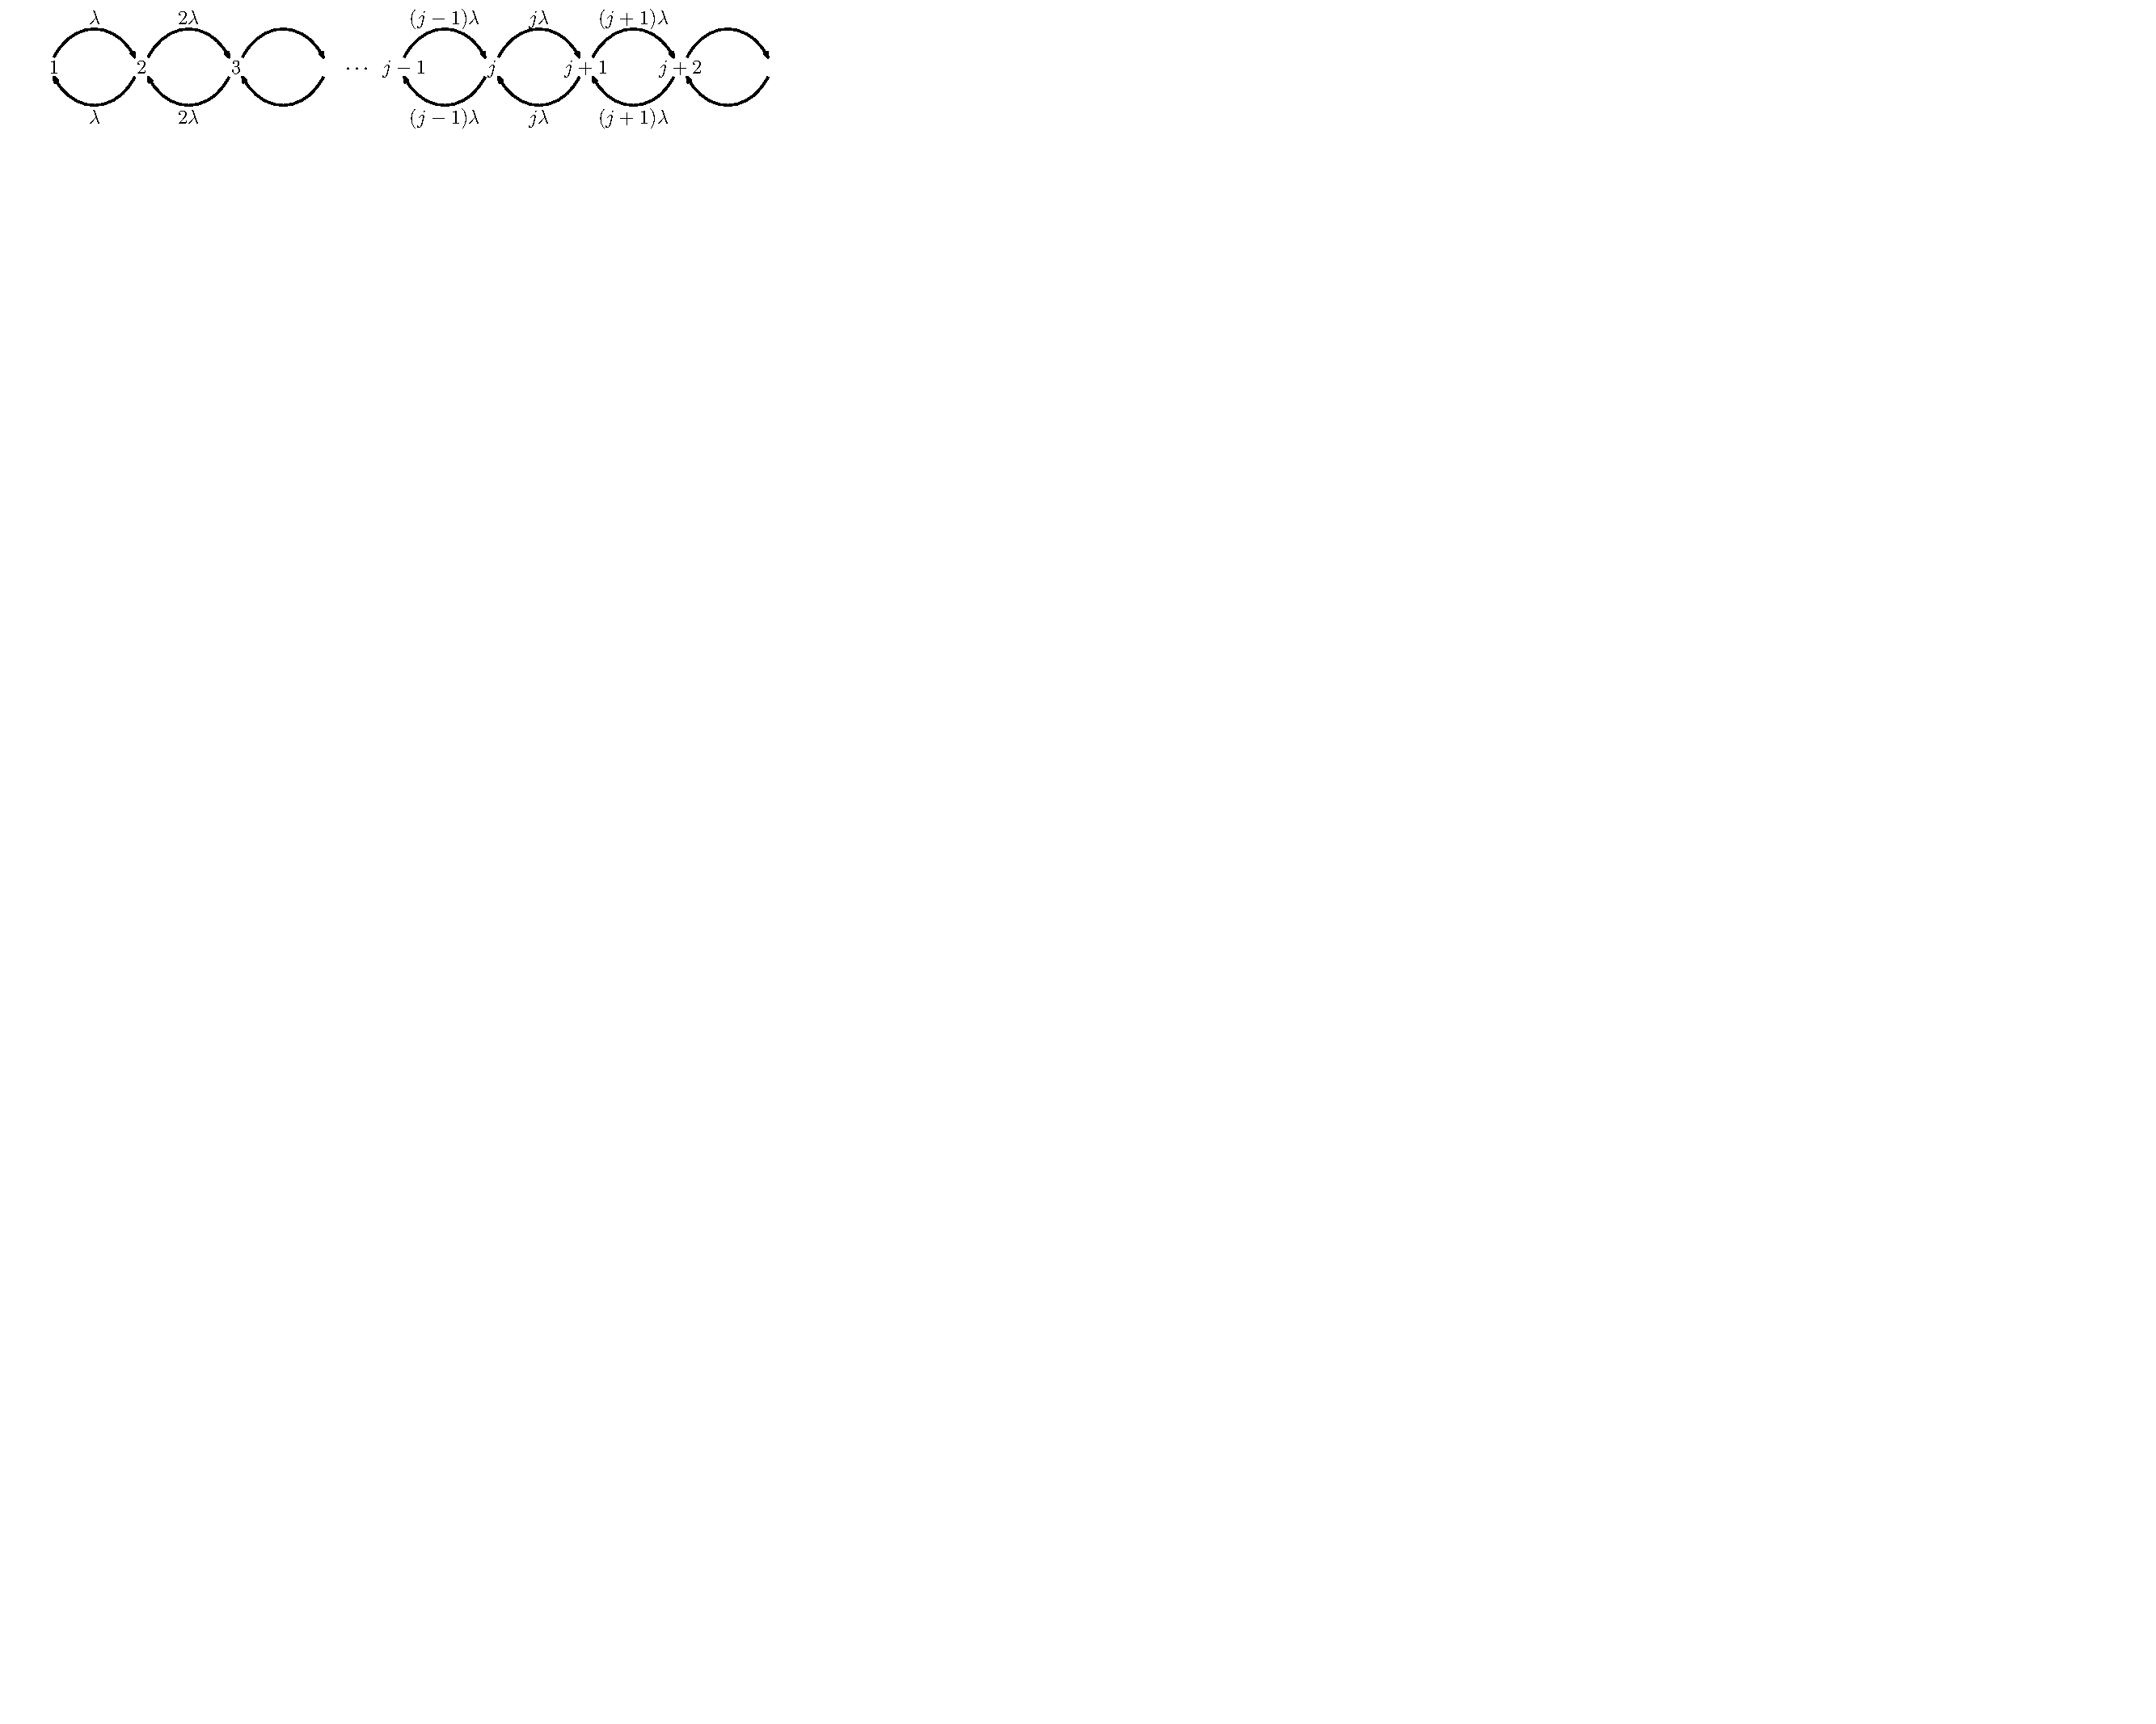
\includegraphics[scale=0.7]{figs/Sagi_fig.pdf}
\caption{Transitions for the process $X_t$}
\label{dpi}
\end{figure}
}%ignore
The process $X_t$ is slightly different than the much-studied critical linear
birth-death process, for which the rate of birth and death from state $j$ are
both equal to $j$ (here the rate of birth is $j$ but the rate of death is
$j-1$), and for which $0$ is an absorbing state (here there are no absorbing
states). However, this stochastic process is essentially a translation of a
critical linear birth-death process with immigration rate equal to the
birth-death rate $\lambda$. This is the key to establishing both parts of the
lemma below. We first define $p_{ij}(t) $ as the transition probability for
$X_t$ to be at state $j$ given that time $0$ it was at state $i$. Note that here
$i$ and $j$ cannot be ignored as they don't specify absolute locations rather
locations relative to a reference gene, i.e., it can be seen that $p_{ij}(t)
\ne p_{(i+r)(j+r)}(t) $. Formally,
\begin{defn}
\label{def-p_ij}
For each ordered pair $i,j \in \{1,2,3\ldots, \}$ let $p_{ij}(t) =
\PP(X_t=j|X_0=i)$. 
\end{defn}

\begin{lemma}
\label{lem-central}
\mbox{}
\begin{itemize}
 \item[(a)] The transition probabilities $p_{ij}(t)$ satisfy the following
 tri-diagonal differential system
 $$ \frac{1}{\lambda}\frac{dp_{ij}(t)}{dt} = -(2j-1)p_{ij}(t) +
 jp_{i(j+1)}(t) +(j-1)p_{i(j-1)}(t),$$
 subject to the initial condition:
 $$p_{ij}(0) = 
 \begin{cases}
 1, \mbox{ if $i=j$}; \\
 0, \mbox{ if $i \neq j$}.
 \end{cases}
 $$
 \item[(b)] The expected value of $X_t$ grows as a linear function of $t$. Specifically,
 $$ \EE[X_t |X_0=i] = i+t \lambda, $$
 Moreover, $X_t$ has no stationary distribution. 
 \item[(c)] Conditional on $X_0=i$, and for fixed value of $t$ and value $B
 >\lambda t$, the probability that the supremum of $X_s$ over the
 interval $[0,t]$ exceeds $B$ is at most $i/(B-\lambda t) \rightarrow
 0$, as $B\rightarrow \infty$.
 \end{itemize}
\end{lemma} 

\begin{proof}

Consider a critical linear-birth death process with immigration $Y_t$, in which
the birth rate and death rate are both equal to $\lambda$, and the immigration
rate is also equal to $\lambda$. Notice that $Y_t$ takes values in $0, 1,2,
\ldots$, in contrast to $X_t$ which takes values from 1 upwards. 

Then the process $Y_t$ is stochastically identical to the process $X_t-1$. To
see this, simply note that both processes are Markovian, and the transition
probabilities for $Y_t+1$ correspond precisely to those indicated in
Fig.~\ref{dpi}. Thus, if we let $\tilde{p}_{ij} := \PP(Y_t =j|Y_0=i).$ $$\PP(X_t
=j|X_0=i) = \PP(Y_t = j-1|Y_0=i-1),$$ and so $$p_{ij}(t) =
\tilde{p}_{i-1j-1}(t). $$

\noindent Now the (tri-diagonal) system of differential equations for
$\tilde{p}_{ij}$ are well-known (see for example Section 6.4.4.\ of
\cite{Allen-book-2011}) and by translation these provide the equations in Part
(a).


For Part (b) observe that:
\begin{equation}
\label{equ}
\EE[Y_t-\lambda t] = \EE[Y_t]-\lambda t = \EE[X_t-1] - \lambda t = \EE[X_t] - 1-\lambda t.
\end{equation}
Now, $Y_t-\lambda t$ is a Martingale process, with $\EE[Y_t-\lambda t] =
\EE[Y_0]$ for all $t\geq 0$. Thus if $X_0=i$ then $$\EE[Y_t-\lambda t] =
\EE[Y_0] = i-1.$$ Combining this with Eqn.~(\ref{equ}) gives $\EE[X_t]= i+
\lambda t$ as claimed.
That $X_t$ has no stationary distribution follows from Theorem 6.1
of~\cite{Allen-book-2011}. 

Part (c) follows by applying the Doob Martingale inequality to the Martingale
process $Y_t-\lambda t$. \qed

\end{proof}

We now set to calculate the probability that a ``non jumping'' gene stays in the
$k$-neighborhood of some reference gene.
Let $q_{ik}(t)$ be the conditional probability that $X_t \in [k]$ (where
$[k]=\{1,2,\ldots, k\}$) given that $X_0=i$. Thus,

\begin{equation}
 \label{eqy0}
 q_{ik} = \sum_{j=1}^k p_{ij}(t).
\end{equation}
In order to state Theorem~\ref{thm-main} we need to define the following
quantity. Let 
\begin{equation}
 \label{eqy}
 q_k(t) := \frac{1}{k}\sum_{i=1}^k q_{ik}(t) =
 \frac{1}{k}\sum_{i=1}^k\sum_{j=1}^k p_{ij}(t).
\end{equation}
In words, $q_k(t)$ is the probability that for {a gene at } an initial state $i$
{(i.e.\ distance from a reference gene)} chosen uniformly at random between 1 and
$k$, the process $X_*$ is still between 1 and $k$ after time $t$ (equivalently,
$q_k(t)$ is the probability that a birth-death-immigration process with all
three rates equal to $\lambda$ and an initial state chosen uniformly at random
between 0 and $k-1$ takes a value at time $t$ that is also at most $k-1$). 

\begin{theorem}
\label{thm-main}
For any given value of $t$, and as $n$ {grows}: $$\overline{SI}(\G_0, \G_t)
\xrightarrow{p} \exp(-2\lambda t)q_k(t),$$ where $\xrightarrow{p}$ denotes
convergence in probability. 
\end{theorem}

\begin{cor}
Thus, if the function $t \mapsto \exp(-2\lambda t)q_k(t)$ has an inverse
$\varphi$ then $$\varphi( \overline{SI}(\G_0, \G_t)) \xrightarrow{p} t$$.
\end{cor}
In particular, for sufficiently large $n$ (including that $\lambda t << n$) one
can use the expression on the left to estimate (an additive) evolutionary
distance and hence construct a tree consistently.

\bigskip

\begin{proof}

We first apply the McDiarmid inequality~\cite{mcdiarmid_1989} to establish that

\begin{equation}
\label{sure}
\overline{SI}(\G_0, \G_t) \xrightarrow{p} \overline{\mu}_t,
\end{equation}
where $\overline{\mu}_t$ is the expected value of $\overline{SI}(\G_0, \G_t)$.

To establish Eqn.~(\ref{sure}) let random variable $N$ denote the total number
of transfer events involving the $n$ genes over the time period of duration $t$.
Then $N$ has a Poisson distribution with mean and variance equal to $\lambda n
t$ and so $N/n$ converges in probability to $\lambda t$. Conditional on $N$, let
$U_1, U_2, \ldots, U_N$ denote the actual sequence of transfer events that take
place, regarding each of these as an arrow from $n$ unlabelled ordered points on
the line to the $n-1$ places that a transfer to be made to (this is illustrated
in Fig.~\ref{3p} in the Appendix for $n=3$, where each of the six single
transfers for $U_i$ are indicated).
\ignore
{
\begin{figure}[htb]
\centering
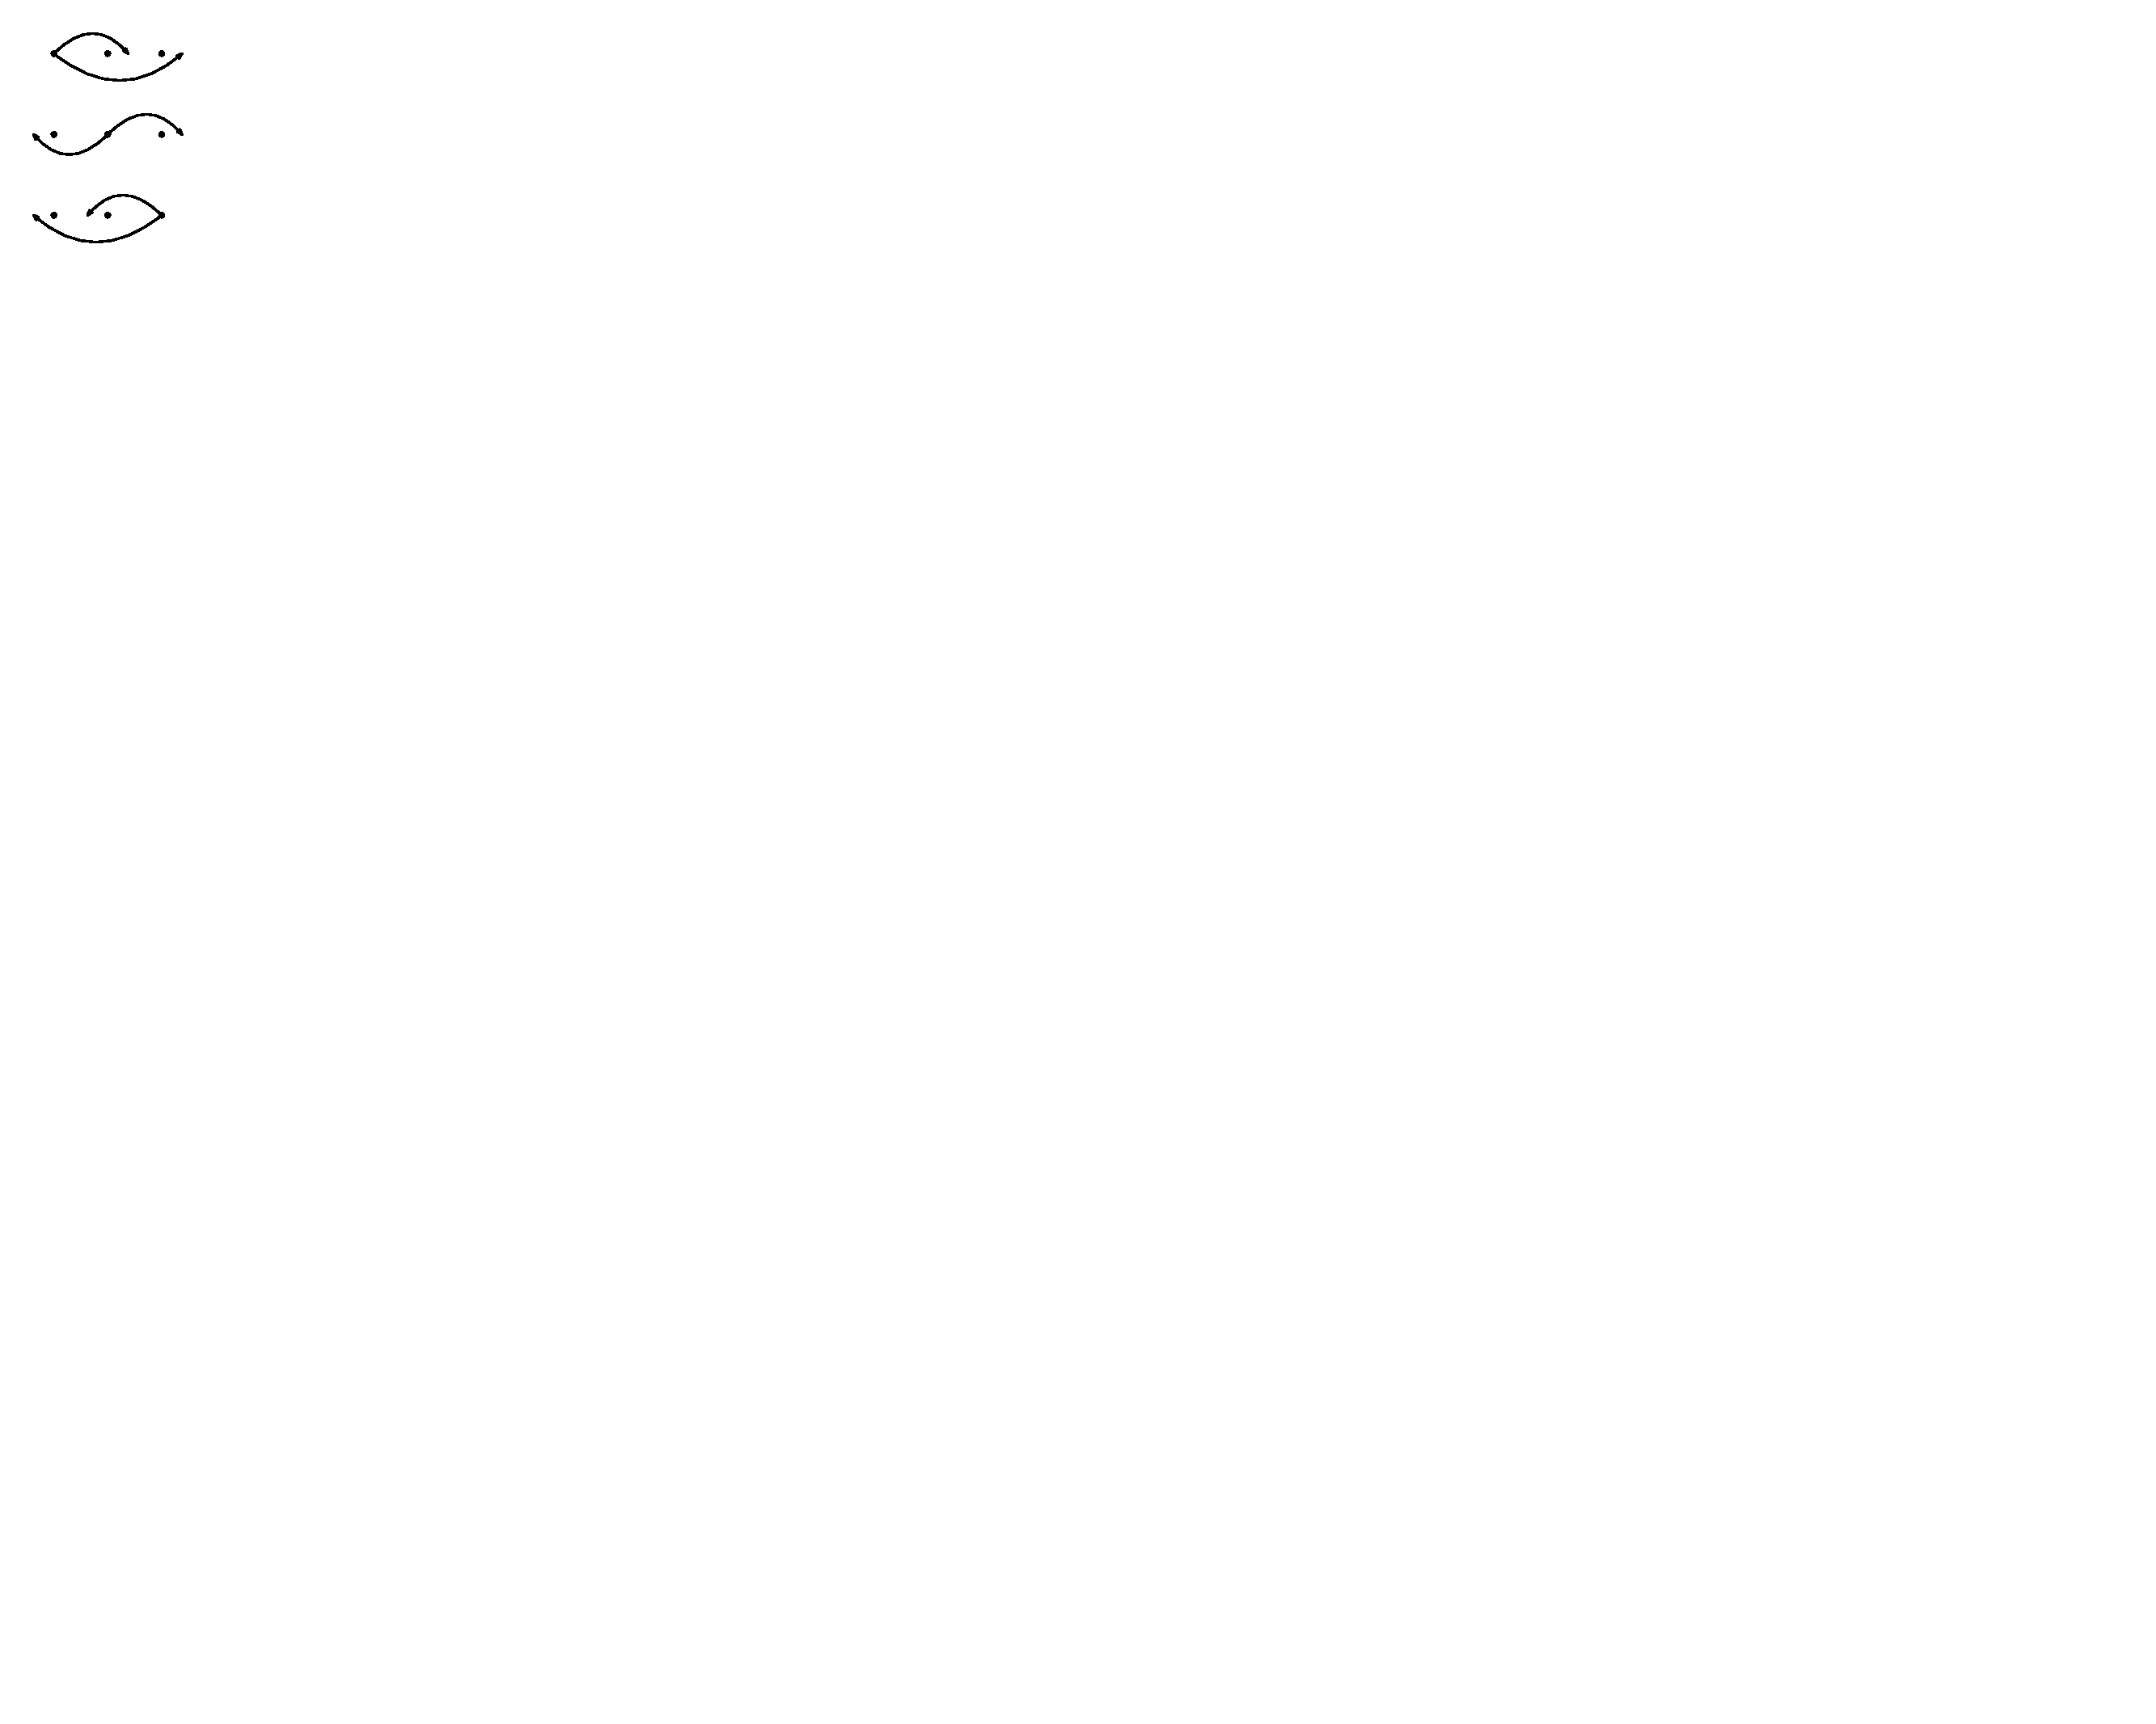
\includegraphics[scale=0.7]{figs/3_dots.pdf}
\caption{The six possible values the random variable $U_i$ can take when $n=3$.}
\label{3p}
\end{figure}
}
These random variables are independent in this model, and $\overline{SI}(\G_0,
\G_t)$ is fully determined by $U_1, U_2, \ldots, U_N$. Moreover, if one of
these transfer events -- say $U_i$ -- were changed to a different transfer event
(say $U'_i$) while keeping the others $U_*$ values the same, then, by the SI
local lemma, $SI_j$ changes for $O(k)$ values of $j$ (and by a maximum of {$6k$}
for each such value) and $\overline{SI}$ changes by at most {$3/n$}. Thus,
conditional on $N$, the McDiarmid inequality implies that the probability that
$\overline{SI}(\G_0, \G_t)$ differs from its expected value $\overline{\mu}_t$
by more than $n^{-\beta}$ is bounded above by: $$
{2\exp\left(-\frac{2n^{-2\beta}}{N(3/n)^2}\right).}$$

If we now select $\beta$ strictly between 0 and $\frac{1}{2}$ and recall that
$N/n$ converges in probability to $\lambda t$, {and since $\lambda t=o(n)$,} it
follows that for all $\epsilon>0$ the probability that $|\overline{SI}(\G_0,
\G_t) - \overline{\mu}_t| > \epsilon$ tends to zero as $n \rightarrow \infty$,
in other words, $\overline{SI}(\G_0, \G_t) \xrightarrow{p} \overline{\mu}_t$, as
claimed.


%%%%%%%%%%%%%%%%%%%

Next, let $\mu_t$ denote the expected value of $SI_j(t)$ for $j$ selected
uniformly at random between k and $n-k$. We have: 
\begin{equation}
\label{mumu}
\overline{\mu}_t= \mu_t,
\end{equation}
by linearity of expectation. Also, for $j$ selected uniformly at random between
$k$ and $n-k$, let $F_j$ be the event that $g_j$ has not been transferred during
the interval $[0,t]$. Under the assumptions of {a Poisson process}, we have:
\begin{equation}
\label{eq2}
\PP(F_j) = \exp(-\lambda t).
\end{equation}
Moreover, we have:
\begin{equation}
\label{novel}
\EE(SI_j(t)|\overline{F_t}) = o(1),
\end{equation}
where $\overline{F_j}$ is the complementary event to $F_j$. Essentially,
Eqn.~(\ref{novel}) says that if a gene in a large genome is transferred to a
random position it is highly unlikely to have any overlap with the genes that it
was previously within distance $k$ of. 


Next, let $W_t$ be {$SI_j(t)$, i.e. $\frac{1}{2k}$ times the number of the $2k$
genes (different from $g_j$) at distance at most $k$ from $g_j$ in $\G_0$ that
also have distance at most $k$ from $g_j$ in $\G_t$}. We {now assume $g_j$ has
not moved (i.e.\ $F_j$), and} claim that:
\begin{equation}
\label{eq3}
\EE[W_t|F_j]= \exp(-\lambda t)q_k(t) +o(1).
\end{equation}


We now establish Eqn.~(\ref{eq3}). For $0< i\leq k$, observe that $g_{j+i}$ is
one of $k$ genes to the right of $g_j$ at time 0. Let $\cE_i(t)$ be the event
that $g_{j+i}$ is within distance $k$ of $g_j$ at time $t$, and let $F_{j+i}$ be
the event that $g_{j+i}$ has not been transferred during the interval $[0,t]$.
By the law of total probability,
\begin{equation}
\label{ppx}
\PP(\cE_i(t)) = \PP(\cE_i(t)|F_{j+i})\PP(F_{j+i}) +
\PP(\cE_i(t)|\overline{F_{j+i}})\PP(\overline{F_{j+i}}).
\end{equation}
Now, $\PP(F_{j+i}) = \exp(-\lambda t)$ and $\PP(\cE_i(t)|\overline{F_{j+i}}) =
o(1)$ and so, from Eqn.~(\ref{ppx}), we have: 
\begin{equation}
\label{ppu}
\PP(\cE_i(t)) = \exp(-\lambda t) \cdot\PP(\cE_i(t)|F_{j+i}) +o(1).
\end{equation}
We now calculate $\PP(\cE_i(t)|F_{j+i})$. Observe first that, conditional on
events $F_j$ and $F_{j+i}$ holding, the gene $g_{j+i}$ is always to the right of
$g_j$ during the interval $[0,t]$. Under the model, $g_{j+i}$ moves one step
closer or further from $g_j$ or stays where it is at any given time. More
precisely, let $r = r(t')$ denote the distance that $g_{j+i}$ is to the right of
$g_j$ at time $t' \leq t$. Then with probability $1-o(1)$, $g_{j+i}$ moves one
step to the left at time $t'$ (towards $g_j$) if one of the $r-1$ genes between
(but not including) $g_j$ and $g_{j+i}$ is transferred at time $t'$, and this
occurs at rate $(r-1)\lambda$. On the other hand, $g_{j+i}$ moves one step to
the right at time $t'$ whenever some gene in the genome is transferred into one
of the $r$ places that available for insertion between $g_j$ and $g_{j+i}$ at
time $t'$. Note that $r$ can be larger than $k$, however, by
Lemma~\ref{lem-central}(c), $r$ is less than $\sqrt{n}$ with probability
$1-o(1)$, and so for this second (right-move) case occurs with rate $\frac{r}{n}
\times (n-r-1)\lambda = r\lambda +o(1)$. 

Thus, the distance that $g_{j+i}$ is to the right of $g_j$ as time goes from $0$
to $t$, behaves asymptotically (as $n \rightarrow \infty$) identically to the
process $X_t$ described above conditioned on starting $X_t$ at state $i$ at time
0 (since $g_{j+i}$ has distance $i$ to the right of $j$ at time 0). In other
words, $\PP(\cE_i(t)|F_{j+i})$ is (asymptotically with $n$) the probability that
$X_t \leq k$ conditional on $X_0=i$, which is the quantity $q_{ik}(t)$ defined
in Eqn. ~(\ref{eqy0}). Thus, $$\PP(\cE_i(t)|F_{j+i}) = q_{ik}(t) +o(1),$$ and
so, for each of the $k$ genes to the right of $g_j$ in $\G_0$ (namely $g_j,
g_{j+1}, \ldots, g_{j+k}$), Eqn.~(\ref{ppu}) gives: $$\PP(\cE_i(t)) =
\exp(-\lambda t)q_{ik}(t) + o(1).$$


An exactly analogous argument applies for the $k$ genes to the left of $g_j$
(i.e.~of the form of the form $g_{j-i}$), leading to the same Equation for
$\PP(\cE_i(t))$. Hence, by linearity of expectation we obtain:
$$\EE[W_t|F_j] = \frac{1}{2k} \sum_{-k \leq i \leq k} \PP(\cE_i(t)) = \exp(-\lambda t)q_{k}(t) + o(1),$$
where $q_k(t)$ is defined in Eqn.~(\ref{eqy}), thereby justifying
Eqn.~(\ref{eq3}).


Next we show that 
\begin{equation}
\label{eq1}
\mu_t =\exp(-2\lambda t)q_k(t) +o(1).
\end{equation}
First, by the law of total expectation we have: $$\mu_t = \EE[
SI_j(t)|F_t]\PP(F_j) + \EE[ SI_j(t)|\overline{F_t}]\PP(\overline{F_j}).$$ Next,
if we apply Eqn.~(\ref{eq2}) and Eqn.~(\ref{novel}) to the first and second
terms (respectively) on the right of this last equation we obtain: $$\mu_t =
\EE[W_t|F_t] \exp(-\lambda t) + o(1) (1-\exp(-\lambda t)),$$ and so, from Eqn.~
(\ref{eq3}), we have: $$ \mu_t = \exp(-\lambda t) \exp(-\lambda t)q_k(t) +o(1) =
\exp(-2\lambda t)q_k(t) +o(1),$$ as claimed.
%%%%%%%%%%%%%%%%%%%%
Combining the pieces from Eqns.~(\ref{sure}), (\ref{mumu}) we have:
$$\overline{SI}(\G_0, \G_t) \xrightarrow{p} \overline{\mu}_t = \mu_t.$$ Now
$\mu_t =\exp(-2\lambda t)q_k(t) +o(1)$ (by Eqn. (\ref{eq1})) and so we obtain
the required convergence in probability: $\overline{SI}(\G_0, \G_t)
\xrightarrow{p} \exp(-2\lambda t)q_k(t)$ as $n \rightarrow \infty$.\qed

This completes the proof of Theorem~\ref{thm-main}.
\end{proof}

\section{Analysis under Real Life Values}
In the previous section we have dealt with asymptotic cases where the size of
the genome goes to infinity and therefore the neighborhood size - $2k$ where $k$
is constant or $o(n)$ - vanishes. However in real life bacterial genomes are of
around 5000 genes and here many relaxations used above do not hold. Therefore,
in order to analyse real data, we must find a realistic model that imitate real
life sizes. Developing analytical results here is substantially harder as the
setting is richer than before. Hence we devised the following approach. We first
simulate the model and try to learn its behavior. Next, we try to fit the
parameters to the model to get the best estimation of the observed behavior. \\
Nevertheless we start with some basic observations that are relevant to this
part for the different settings than before. The following basic observation is
given without proof.
\begin{observation}
\label{obs-SI-as-prob}
Under the uniform jump model, for genes $g_i, g_j$ such that $g_i \in N_{2k}
(g_j,\G(0))$,
$$SI=\PP(g_i \in N_{2k}(g_j,\G(t)).$$
\end{observation}

The next simple lemma gives an upper bound on SI when $t\rightarrow \infty$. We
will use it during our simulation study to provide a scaling factor to the
inferred function.
\begin{lemma}
\label{lem-SI-upper-bound}

Under the uniform jump model, when $t\rightarrow \infty$
$SI= 1-\frac {2k}{n-1} $
\end{lemma}
\begin {proof}
There are $2k$ genes in gene $g_i$'s original neighborhood $N_{2k}(g_i,\G(0))$.
These are scattered uniformly in $\G(\infty))$ and hence also in
$N_{2k}(g_i,\G(\infty))$. Therefore in particular the expected number of these
genes in $N_{2k} ( g_i,\G(\infty) )$ is $\frac {2k}{n-1} $ and the result
follows. \qed
\end {proof}


\subsubsection{The Linear Model.}

We start with a simple case that will serve as the basis for the subsequent
development. We first define the following.
\begin{defn} 
\label{def-DEA}
The {\em disjoint events assumption} (DEA) assumes that a transferred gene $g_i$
leaves its original, unviolated neighborhood and lands at a new, unviolated
neighborhood.
\end{defn} 
In other words, under DEA, all neighborhoods associated with transfer events are
disjoint. We note that such an assumption violates the randomness of our model
as we cannot assume this under a random model. Nevertheless it holds with high
probability for small $t$, i.e., between closely related species. 

It is easy to see that under DEA, Lemma~\ref{lem-local} - the SI local lemma
holds in equality and therefore the contribution of each event to SI is
approximately $\frac 3n$. Hence, under DEA, for relatively small number of HGT
events $N$, the expected SI is $\frac {3N}n$.


\subsubsection{The Expanded Model.} 

As the DEA, and hence linearity of SI, holds for a relatively short time, we set
to develop a more realistic model that also considers non-disjoint events. As
discussed above the goal here is not to find an exact model as in the asymptotic
model of Section~\ref{sec-asymptotic}, rather to find a sound approximation to
it. The first approach then is to obtain intuition via simulation study.
To this end, two identical genomes, $G_1$, $G_2$, were created. Then, iterations
of HGT events were executed. In each iteration one gene was randomly chosen from
$G_2 $ and relocated to a random position in $G_2$. After each HGT event, the SI
distance between the two genomes was calculated. Figure~\ref{fig-simul}(a)
illustrates the outcome of our simulation by showing SI as a function of the
number events, for various $k$'s. Also, the theoretical linear model is
presented, and we can see that this model (which assumes disjoint events, DEA)
departs from the simulation results after about $200$ events ($20\%$ of the
genome size) or less, depending on $k$.  Interestingly, as was shown
theoretically (Lemma~\ref{lem-local}), this line is independent of $k$. Also, we
can see that the maximum value of SI behaves according to
Lemma~\ref{lem-SI-upper-bound}. In Figure~\ref{fig-simul-vs-model}(a) of
Appendix~\ref{sec-append-pw}, we also present a pairwise simulation, but here we
present the standard deviation (SD) of SI as a function of the number of HGT
events. Here we can see that the first few events cause a rapid increase in SD,
then SD starts to decrease in a logarithmic manner. The place where SD comes to
its maximum value has interesting meaning which will be discussed later.


\begin{figure}[tb]
\begin{center}

\begin{tabular}{cc}
\hspace{-1.5cm}
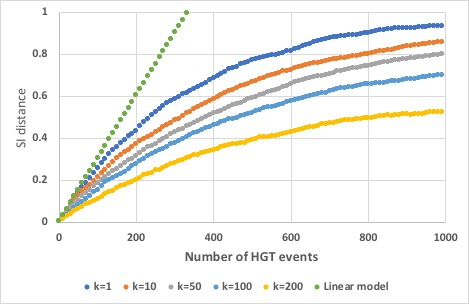
\includegraphics[width = 3.7in,angle=0]{figs/simul.jpg} &
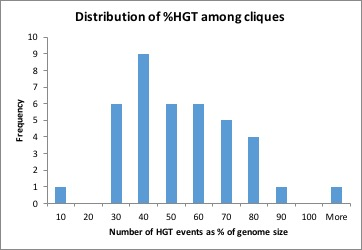
\includegraphics[width = 3.5in,angle=0]{figs/real-data-HGT-distr.jpg} \\
% \hspace{-2.5in}
 (a) & %\hspace{-3in} 
 (b) 
\end{tabular}
\caption{\small (a) {\bf Results of pairwise simulation between two genomes:} SI
as a function of number of HGT events. $G_0$ and $G_1$ were created identically
with 1000 genes. Next, iteratively, a gene $g_i$ was randomly chosen from $G_1$
and relocated to a random position in $G_1$. After each HGT event
$\overline{SI}(\G_0, \G_1)$ was calculated and is displayed as a function of
number HGT events, for various sizes of k. Also, the theoretical linear model is
presented in green. (b) {\bf Distribution of \%HGT (relative to genome size)
among cliques}. In each clique of closely related species we calculate the SI
between each pair of species. Then we calculate the predicted number of HGT
events with the practical model we developed (Eqn.~(\ref{eq-final-SI-simul})), and
averaged this value for each clique. Here we present the distribution of this
value among cliques.
\label{fig-simul}}
 \end{center}
\end{figure}

As can be perceived from Figure~\ref{fig-simul}(a), all curves follow a
logarithmic shape implying that the increase follows an \emph{ exponential
decay}. A quantity is subjected to exponential decay (or growth) if it proceeds
at a rate proportional to its current value, i.e., $\frac{dN}{dt}=\Lambda N$,
where $N$ is the quantity measured, $t$ is time, and $\Lambda < 0$ is the decay
constant~\cite{durrett2008probability}. Our goal is to have an expression for
the expected change in SI after $m$ HGT events. This is important since by
integrating this expression we get the expected value of SI, $\EE[SI]$,
resulting from HGT events. We will denote this target expression as $\frac
{d}{dt}\EE[SI]$, since this is the derivative of $\EE[SI]$. A further goal here
is to develop more of an intuition and determine how to set the actual
parameters tracing the simulation best.\\ We start by noting that the HGT events
are distributed uniformly throughout the genome. Considering this, we start by
finding, how many events are required for each gene $g_i$ to have an SI score of
$\frac 1{2k}$ (and hence total SI of $\frac 1{2kn}$). To tackle this question,
we assume most of the events conform with DEA, as the events are uniformly
distributed and genomes are relatively close - the process is at the beginning
(see Figure~\ref{fig-simul}(a)).

\begin{observation}
After $\frac n{6k}$ events, the expected SI at every gene $g_i$, and hence the
total SI, is $\frac 1{2k}$.
\end{observation}
\begin{proof}
We can look at the genome as a sequence of $\frac n{2k}$ adjacent
$2k$-neighborhoods. By Lemma~\ref{lem-SI-upper-bound}, under DEA each event
contributes $\frac{ 6k}{2kn}=3/n$ to the total SI. Hence, under uniform
distribution, we get that after $\frac n{6k}$ events the expected number of
events occurring at a neighborhood is $1/3$ yielding $\frac n{6k}\frac 3n =
\frac1{2k}$ contribution to the total SI, and the lemma follows. \qed

\end{proof}
\begin{lemma}\label{lem:dea}
If each gene contains $m$ violations, the addition to the SI score resulting
from the next event is $\frac{6k-3m}{2kn}$.
\end{lemma}
A proof can be found in Appendix~\ref{sec-append-lem}.

We found that the contribution of the next event, after $m\frac n{6k}$ events is
$\frac {6k-3m}{2kn} = \frac 3n-\frac{3m}{2kn}$. This means that the change in
the contribution to SI for each period of $n/(6k)$ events, is $ \left (\frac
3n-\frac{3m+3}{2kn}\right )-\left ( \frac 3n-\frac{3m}{2kn}\right ) =
-\frac{3}{2kn}$. Having proved that, we recall that the quantity $N$ being
measured is $\frac d{dt}\EE(SI)$, so the expression $\frac {d N}{dt}$ that
changes over time (or HGT events), is $\frac {d^2}{dt^2}\EE(SI)$. We found that
for time period of $\frac n{6k}$ events, $\frac{d^2}{dt^2}\EE(SI) = -
\frac{3}{2kn}$ and this is $\frac{d N}{dt}$ for this time period. Now, recall
that under exponential decay, $\frac{d N}{dt} = \Lambda N$ so in order to find
$\Lambda$ we write 
\begin{equation}
\Lambda = \frac{\frac {d N}{dt}}{N} = \frac {-\frac 3{2kn}}{\frac
3n-\frac{3m}{2kn}} \approx \frac {-\frac {3}{2kn}}{\frac 3n} = -\frac 1{2k}.
\end{equation}

A similar procedure for the next time periods (i.e.\ for having expected
violations $2$, $3$, etc.\ will yield, as long as $\frac 3n >> -\frac{3m}{2kn}$,
the same $\Lambda = -\frac 1{2k}$, as indeed required by such growth
(exponential). As this derivation is involved, the table in
Figure~\ref{fig-SI-contr-tab} (see Appendix) provides manual derivation for the
initial steps of $1,2,3$ violations per neighborhoods, demonstrating the
constancy of decay rate $\Lambda = -\frac 1{2k}$. Of course this analysis is
quite crude and by no means provides a rigorous proof for the exponential decay,
as this should be significantly harder even than the asymptotic case.
Nevertheless it provides us with intuition and insight of what are the
parameters to the decay function as we next show. First, we note that the
$\Lambda = -\frac 1{2k}$ obtained is aggregated over an entire time period of
$\frac n{6k}$ events, so in order to put it in the formula we need to divide
$\Lambda $ by this factor, $\frac n{6k}$ yielding,

\begin{equation}
\Lambda^* = \frac \Lambda {\frac n{6k}} = \frac {-\frac 1{2k}}{\frac
 n{6k}} = -\frac 3n.
\end{equation}

Now we can plug it into the exponential decay function: $N_t=N_0e^{\Lambda^*
t^*}$ where $t^*$ in our case is the number of events, in our case $\lambda t$.

\begin{equation}
\label{eq-E-SI'}
\frac d{dt}\EE[SI]=\frac 3ne^{-\frac 3n\lambda t}.
\end{equation}

In order to obtain $\EE[SI]$ we need to integrate Eqn.~(\ref{eq-E-SI'}), yielding
$\EE[SI]=1 - e^{-\frac {3}{n}\lambda t}$. Now, as $n$ is finite here, the latter
tends to one as $t\rightarrow\infty$. However, recall that by
Lemma~\ref{lem-SI-upper-bound} SI is bounded from above by $1-\frac {2k}{n-1}$
so we treat this as a scaling factor for our decay function. Our final
refinement concerns with cases of relatively large neighborhoods (e.g. $k=100,
200, 300, 400$) taking in consideration the case the gene transferred into its
original neighborhood, as was shown above to be $\frac {3-\frac {5k}{n-1}}{n}$
instead of $3/n$. Therefore we obtain:

\begin{equation}
\label{eq-final-SI-simul}
\EE[SI]=\left (1-\exp\left (-\frac {3-\frac
 {5k}{n-1}}{n}\lambda t\right ) \right )\left (1-\frac{2k}{n-1} \right ).
\end{equation}

Although this study is not as rigorous as the asymptotic case, its strength is
by considering practical values as found in nature. Indeed in
Figure~\ref{fig-simul-vs-model}(b) we show the performance of this model compare
to simulated data for various values of $k$. As can be seen, even for very large
neighborhood size ($k$), prediction (of \#HGTs) remains quite accurate and this
is due to the refinement of incorporating $k$ into the exponent.



\subsection{Result on Real Microbial Data}
Once we found a plausible model for relevant sizes, we aimed at using it to
infer HGT activity in microbial data. We used the EggNOG
database~\cite{Powell12} that is the largest, unbiased, orthology database,
containing protein sequences of 1133 species, most of them bacteria. In
addition, this database clusters all proteins into COGs (Clusters of Orthologous
Groups)~\cite{Tatusov-COGS}. This means that an organism is represented as a
list of COG names ordered by their order of appearance in its genome. In order
to work only in the valid region, i.e.,  avoid ``1'' entries in our matrix, we
removed from the matrix all entries above a threshold (specifically SI $\ge
0.95$) and in the resulted matrix searched for largest cliques. This has yielded
39 cliques (subsets) or bacteria, conforming with the conventional partition
into {\em genera} (data not shown).

Figure~\ref{fig-simul}(b) gives an overview on the distribution of the relative
number of HGTs among the cliques. For a detailed account, we provide a table in
Appendix~\ref{sec-append-table} (see Figure~\ref{fig-real-data-table}) which
lists for each such clique, its corresponding genus, its average SI, and the
average number (in terms of percentage of the average genome size (\# genes)) of
HGT events separating between each pair of	species in that clique.  We found
that this parameter is normally distributed (Shapiro-Wilks test:
$p=0.238$)~\cite{Shapiro-Wilks-book} with mean of $52.7\%$, median of $54.1\%$
and SD of $23.78\%$. In other words, we found that the average number of HGT
events between pairs of species inside a genera is about $50\%~(\pm 20)$ of the
genome size. We believe this is an interesting finding that cannot be readily
obtained by standard HGT methods as constructing species trees within genera is
not trivial. Moreover, the fact that the SI values themselves are not normally
distributed (Shapiro-Wilks test: $p=0.024$) intensifies the soundness of this
finding.

\section{Discussion}
In this paper we have provided a first statistical modeling for the {\em synteny
index} (SI) as a phylogenetic marker. The major advantage of SI is that it
combines both gene order and gene content evolutionary signals. The latter
allows not only a comparison between genomes over different gene sets, a
pervasive phenomenon in prokaryotes, rather comparing the order of their shared,
core, gene set, a signal that is ignored by content-based approaches.

Statistical parametric approaches are nowadays widely accepted as the method
of choice in a host of applications in biology. Starting from Felsenstein's
seminal demonstration of the statistical inconsistency of maximum
parsimony~\cite{FELSENSTEIN78} and his subsequent remedy to this
flaw~\cite{felsenstein1981evolutionary}, maximum likelihood is now a gold
standard also in phylogenetics and most popular
packages~\cite{Swofford81,PHYLIP,PhyML-systBiol-2010} offer a likelihood based
solution. These approaches rely on a single gene that is conserved among all
taxa and hence is appropriate for comparison. Such genes however are to
conserved and do not furnish a strong enough signal.

In contrast, gene-based (gene order and content) approaches were found to
provide enough signal allowing more resolved trees~\cite{Wolf-BMC-2001}.
Nevertheless, although such approaches exist for several decades already, to the
best of our knowledge, no detailed model, showing additivity and consistency
under HGT, was proposed. Similarly, while the usefulness of SI was proved
empirically in previous works~\cite{Shifman13,Adato-PLOSCB-2015}, no analytical
proof for it correctness was shown. Therefore, the above discussion emphasises
the importance of the direction we took in this work -- laying the groundwork for
gene based models phylogenetics.

As this work has just handled the most basic case -- the jump model --
extensions to more advanced models such as {\em the indel model} in which new
genes are added to the genome, but at an equal rate of gene loss, so genome
sizes is approximately fixed. Another natural extension is considering transfer
of cluster of genes, forming {\em genomic islands}~\cite{Koonin-JCB-2011}.
Therefore we believe that the tools developed here will serve as the basis for
such further extensions. 

\clearpage


\bibliographystyle{abbrv}

\bibliography{aes2e}
%\eject\vfill
\clearpage

\appendix
\section{ Optional extra material}
In this part we provide farther information and proofs to claims
remained outside due to space considerations.

\subsection{Describing $q_k(t)$}


\mbox{}


Recall that $q_{ik}(t)$ is the conditional probability $ \PP(X_t \in [k]|X_0=i)$
(where $[k]=\{1,2,\ldots, k\}$, and $p_{ij}(t)$ is the probability that the
random walk $X_t$ (described above) is in state $j$ after duration $t$,
conditional on $X_0= i$. Thus, $q_{ik}(t)= \sum_{j=1}^k p_{ij}(t)$, and so:
$$\frac{dq_{ik}(t)}{dt} = \sum_{j=1}^k \frac{dp_{ij}(t)}{dt}.$$

\begin{lemma}
\begin{equation}
\label{stro}
\frac{dq_{ik}(t)}{dt} = k \lambda [p_{i(k+1)}(t)-p_{ik}(t)].
\end{equation}
\end{lemma}
\begin{proof}
Lemma~\ref{lem-central}(a) gives: $$\frac{1}{\lambda}\frac{dq_{ik}(t)}{dt} =
\sum_{j=1}^k -(2j-1)p_{ij}(t) + jp_{i(j+1)}(t) +(j-1)p_{i(j-1)}(t).$$ and we
show that the term on the right is simply $k [p_{i(k+1)}(t)-p_{ik}(t)]$ by
induction on $k$. The base case $k=1$ gives
$\frac{1}{\lambda}\frac{dq_{ik}(t)}{dt} = p_{i(k+1)}(t)-p_{ik}(t)$ as claimed.
For the induction step, observe that: $$\sum_{j=1}^{k+1} \frac{dp_{ij}(t)}{dt}
=\sum_{j=1}^k \frac{dp_{ij}(t)}{dt} +\frac{dp_{i(k+1)}(t)}{dt},$$ and by the
inductive hypothesis the first term equals $k \lambda [p_{i(k+1)}(t)-p_{ik}(t)]$
while by Lemma~\ref{lem-central}(a)) the second term equals $\lambda$ times
$-(2k+1)p_{i(k+1)}(t) + (k+1)p_{i(k+2)}(t) + kp_{ik}(t)$. Adding these two terms
together gives $(k+1) \lambda [p_{i(k+2)}(t)-p_{i(k+1)}(t)]$, which establishes
the induction step, thereby justifying Eqn.~(\ref{stro}). \qed
\end{proof}

Recall (from Eqn.~(\ref{eqy})) that $q_k(t) = \frac{1}{k}\sum_{i=1}^k
q_{ik}(t)$. It now follows that: $$\frac{dq_{k}(t)}{dt} = \frac{1}{k}
\sum_{i=1}^k \frac{dq_{ik}(t)}{dt} =\lambda \sum_{i=1}^k
[p_{i(k+1)}(t)-p_{ik}(t)].$$

In particular,

$$\frac{d}{dt} \exp(-2\lambda t)q_k(t) = \lambda \exp(-2\lambda t)\left[-2q_k(t)
+ \sum_{i=1}^k [p_{i(k+1)}(t)-p_{ik}(t)]\right],$$

\noindent and so the claim that $\exp(-2\lambda t)q_k(t)$ is monotone decreasing
(and so the function $\varphi$ is well-defined) amounts to verifying that
\begin{equation}
\label{eqo}
\sum_{i=1}^k \left( p_{i(k+1)}(t)-p_{ik}(t) -2 \left( \sum_{j=1}^k p_{ij}(t)
\right)\right)<0.
\end{equation}

\subsection{Proof of Lemma~\ref{lem:dea}}\label{sec-append-lem}

\begin{proof}
We will show this holds for any $m<2k$. Having $m$ violation in each gene's
neighborhood, means that each gene has SI score of $\frac{2k-m}{2k}$, that is,
each gene is missing $m$ of its original neighbors. Let us consider the next
event, as some gene $g_i$ is jumping to a new neighborhood. First, gene $g_i$,
as all other genes, is missing $m$ old neighbors. That is, when making this
jump, it loses its remaining $2k-m$ neighbors, and also, these $2k-m$ genes are
losing gene $g_i$ as their old neighbor. That is, $\frac{2(2k-m)}{2kn}$
contributions to the SI score. Now, in the new neighborhood of gene $g_i$, there
are $2k$ genes that are now having $g_i$ in their current neighborhood. Each of
these genes is already missing $m$ old neighbors. For each of these genes, the
probability that gene $g_i$ pushed out of the neighborhood an old neighbor is
$\frac{2k-m}{2k}$. When this is the case, there is a contribution of
$\frac1{2kn}$ to the SI score. So, for the new neighborhood contribution
calculation we have: the number of potential genes in the new neighborhood times
the probability they lose a neighbor $\frac{2k-m)}{2k}$ times the change in the
SI from this loss $\frac{1}{2kn}$. That is, $\frac{2k(2k-m)}{2k }\frac{1}{2kn} =
\frac{2k-m}{2kn}$. Summing the contribution from the old and new neighborhoods
and the jumping gene $g_i$ we end with $\frac{3( 2k-m ) }{2kn} =
\frac{6k-3m}{2kn}$ contribution to the total SI score. \qed
\end{proof}
\clearpage

\section{Auxiliary Data and Figures}
In this section of the Appendix we provide further details and illustrations to
summaries provided in the main text.

\subsection{Further results of pairwise simulation between two
genomes}\label{sec-append-pw}

\begin{figure}[h]
\begin{center}

\begin{tabular}{cc}
\hspace{-1.5cm}
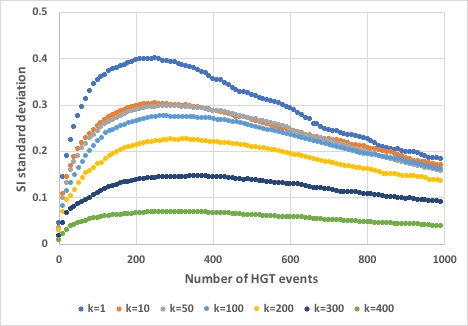
\includegraphics[width = 3.5in,angle=0]{figs/simul-sd.jpg} &
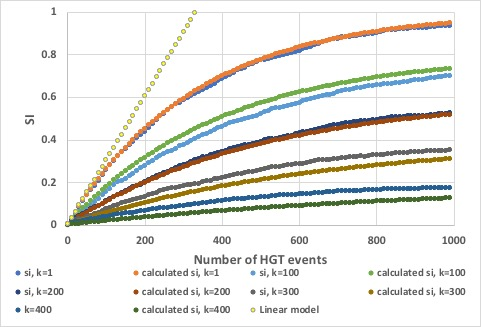
\includegraphics[width = 3.7in,angle=0]{figs/simul-vs-model.jpg} \\
% \hspace{-2.5in}
 (a) & %\hspace{-3in} 
 (b) 
\end{tabular}
\caption{\small (a) Standard deviation (SD) of $\overline{SI}(\G_0, \G_1)$ is
displayed as a function of number of HGT events, with different size of k. We
can see that the first few events cause a rapid increase in SD, then SD
decreases in a logarithmic manner.
(b) Here we present the same simulation as in Figure~\ref{fig-simul}(a), but we
added the result of the theoretical SI calculated by our suggested model
(Eqn.~(\ref{eq-final-SI-simul})). As can be seen, although the neighborhood size
becomes a significant part of the genome size, performance is still fairly
accurate. 
\label{fig-simul-vs-model}}
 \end{center}
\end{figure}

\subsection{The Gene Neighborhood as a Markov Chain}
%\ignore
{
\begin{figure}[htb]
\centering
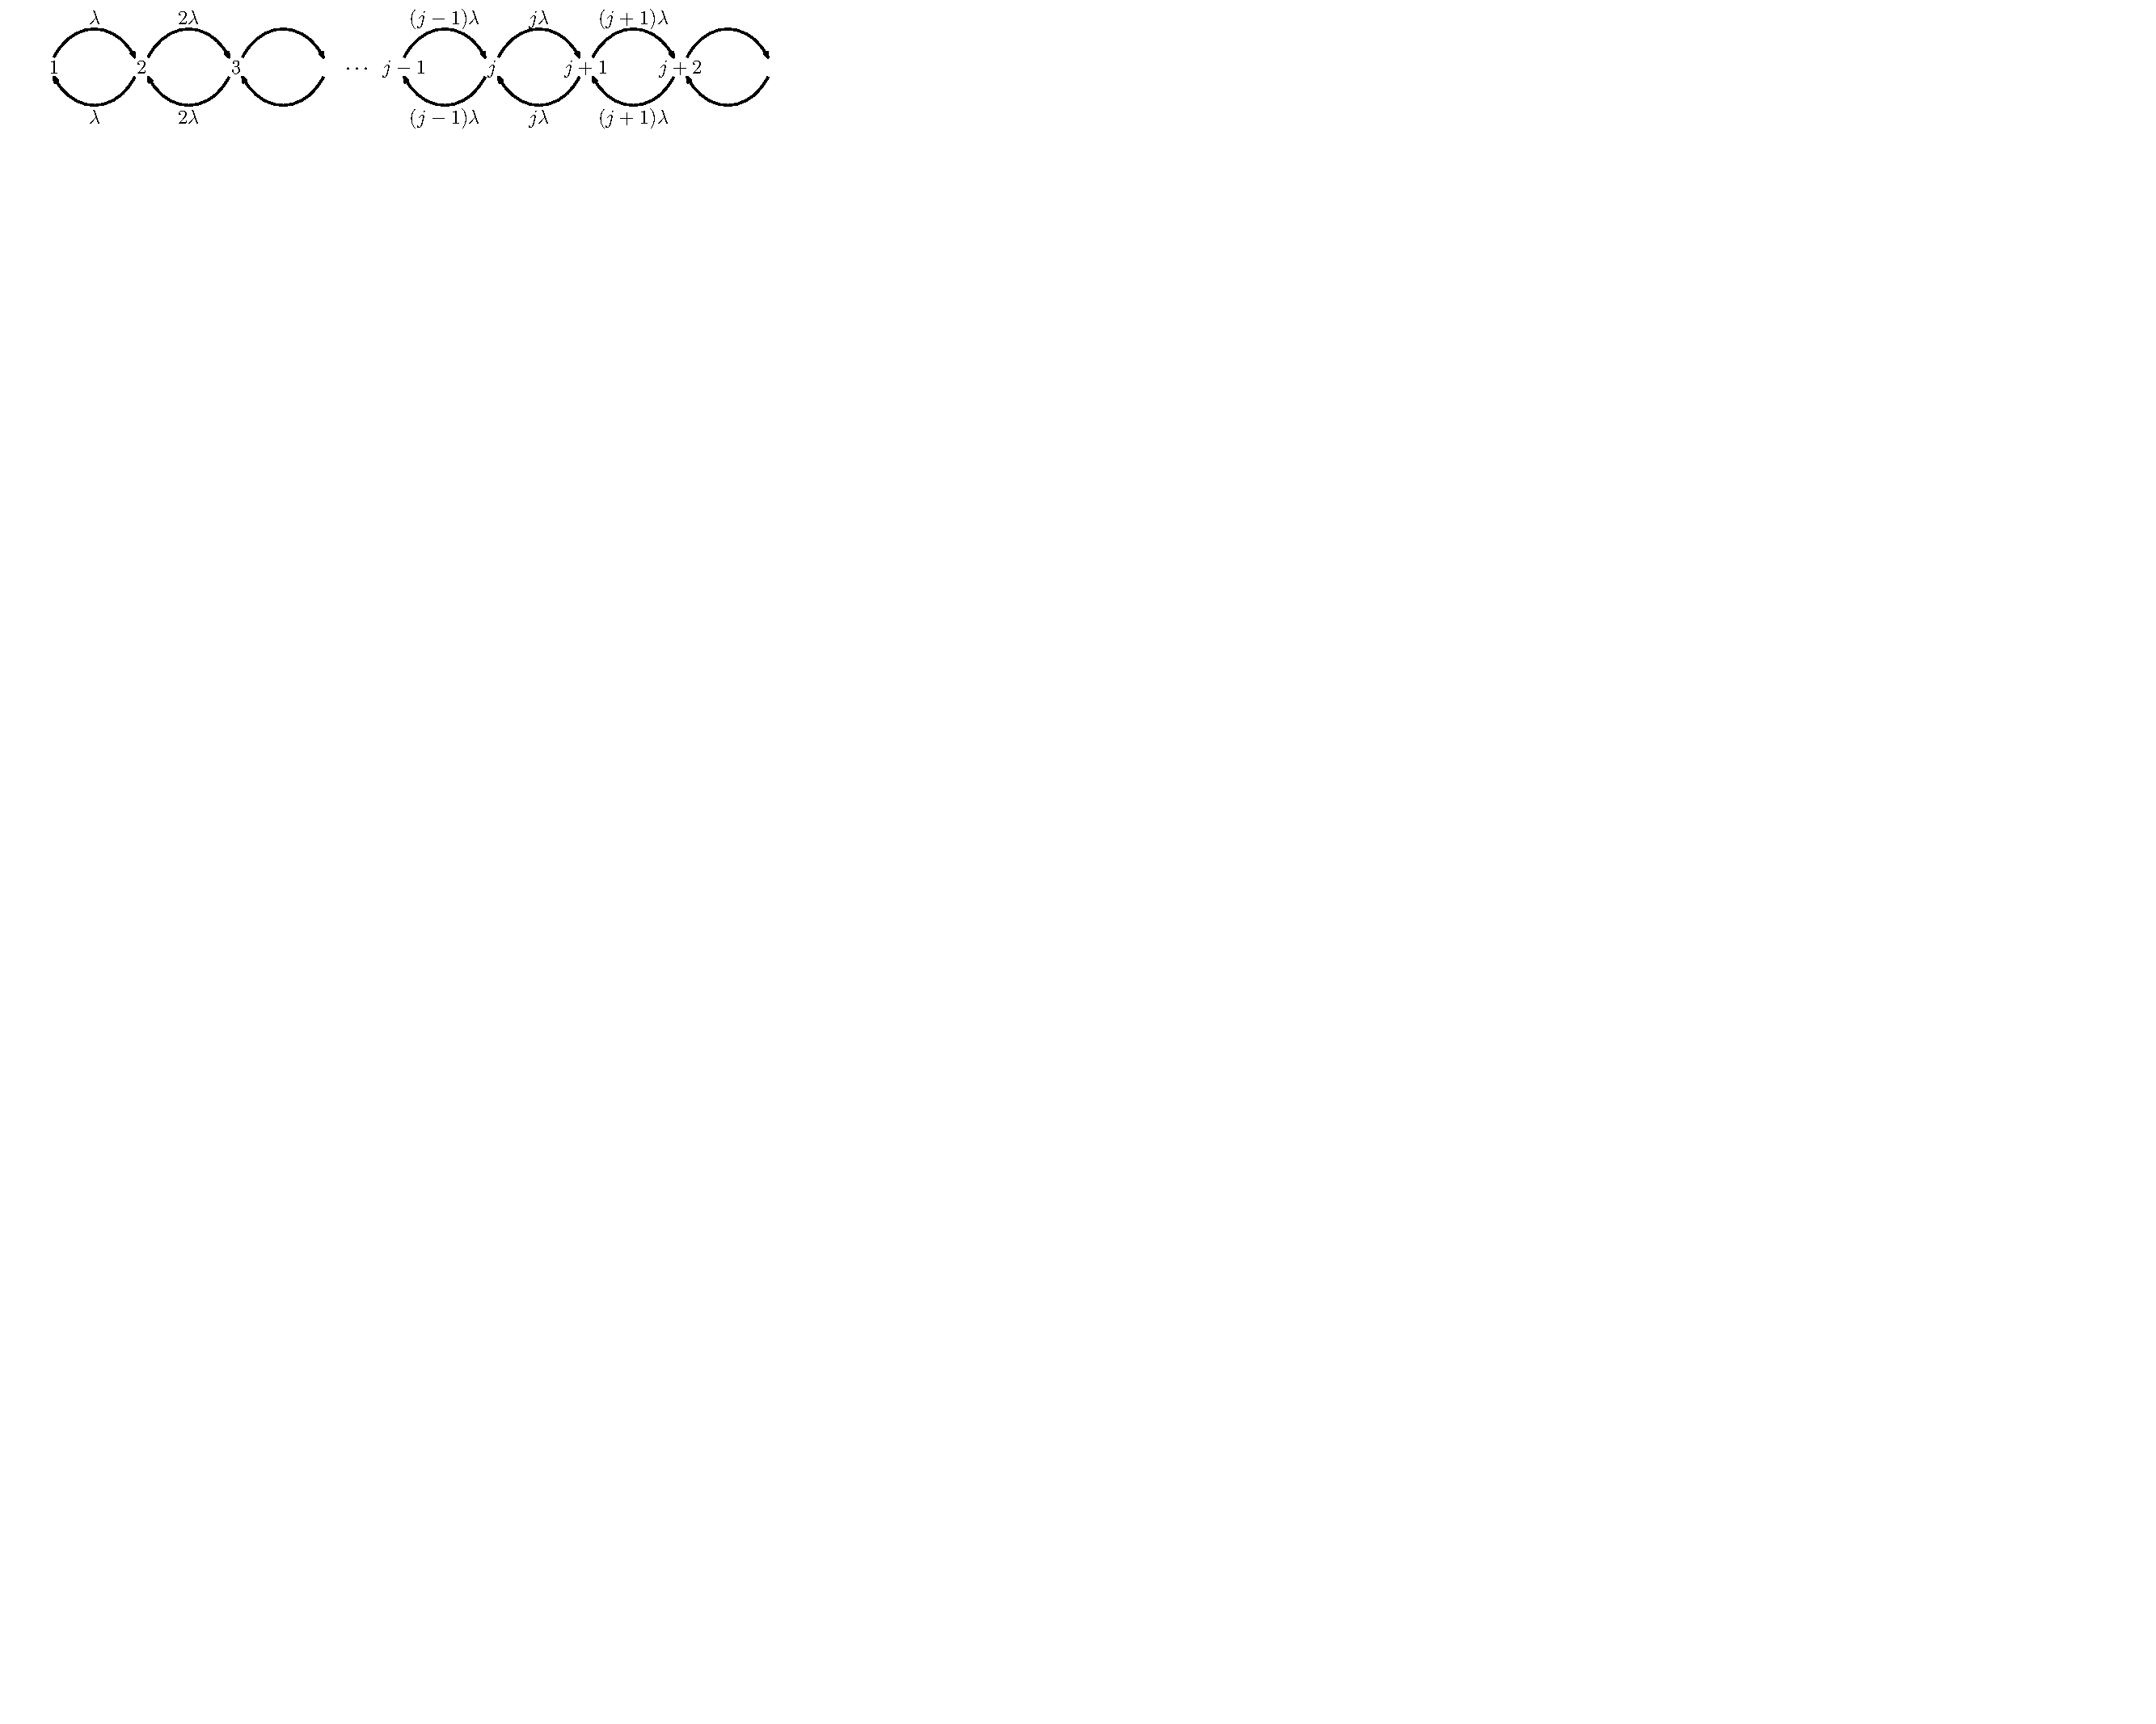
\includegraphics[scale=0.7]{figs/Sagi_fig.pdf}
\caption{Transitions for the process $X_t$}
\label{dpi}
\end{figure}
}%ignore


\subsection{The State Space of the Random Walk}
%\ignore
{
\begin{figure}[htb]
\centering
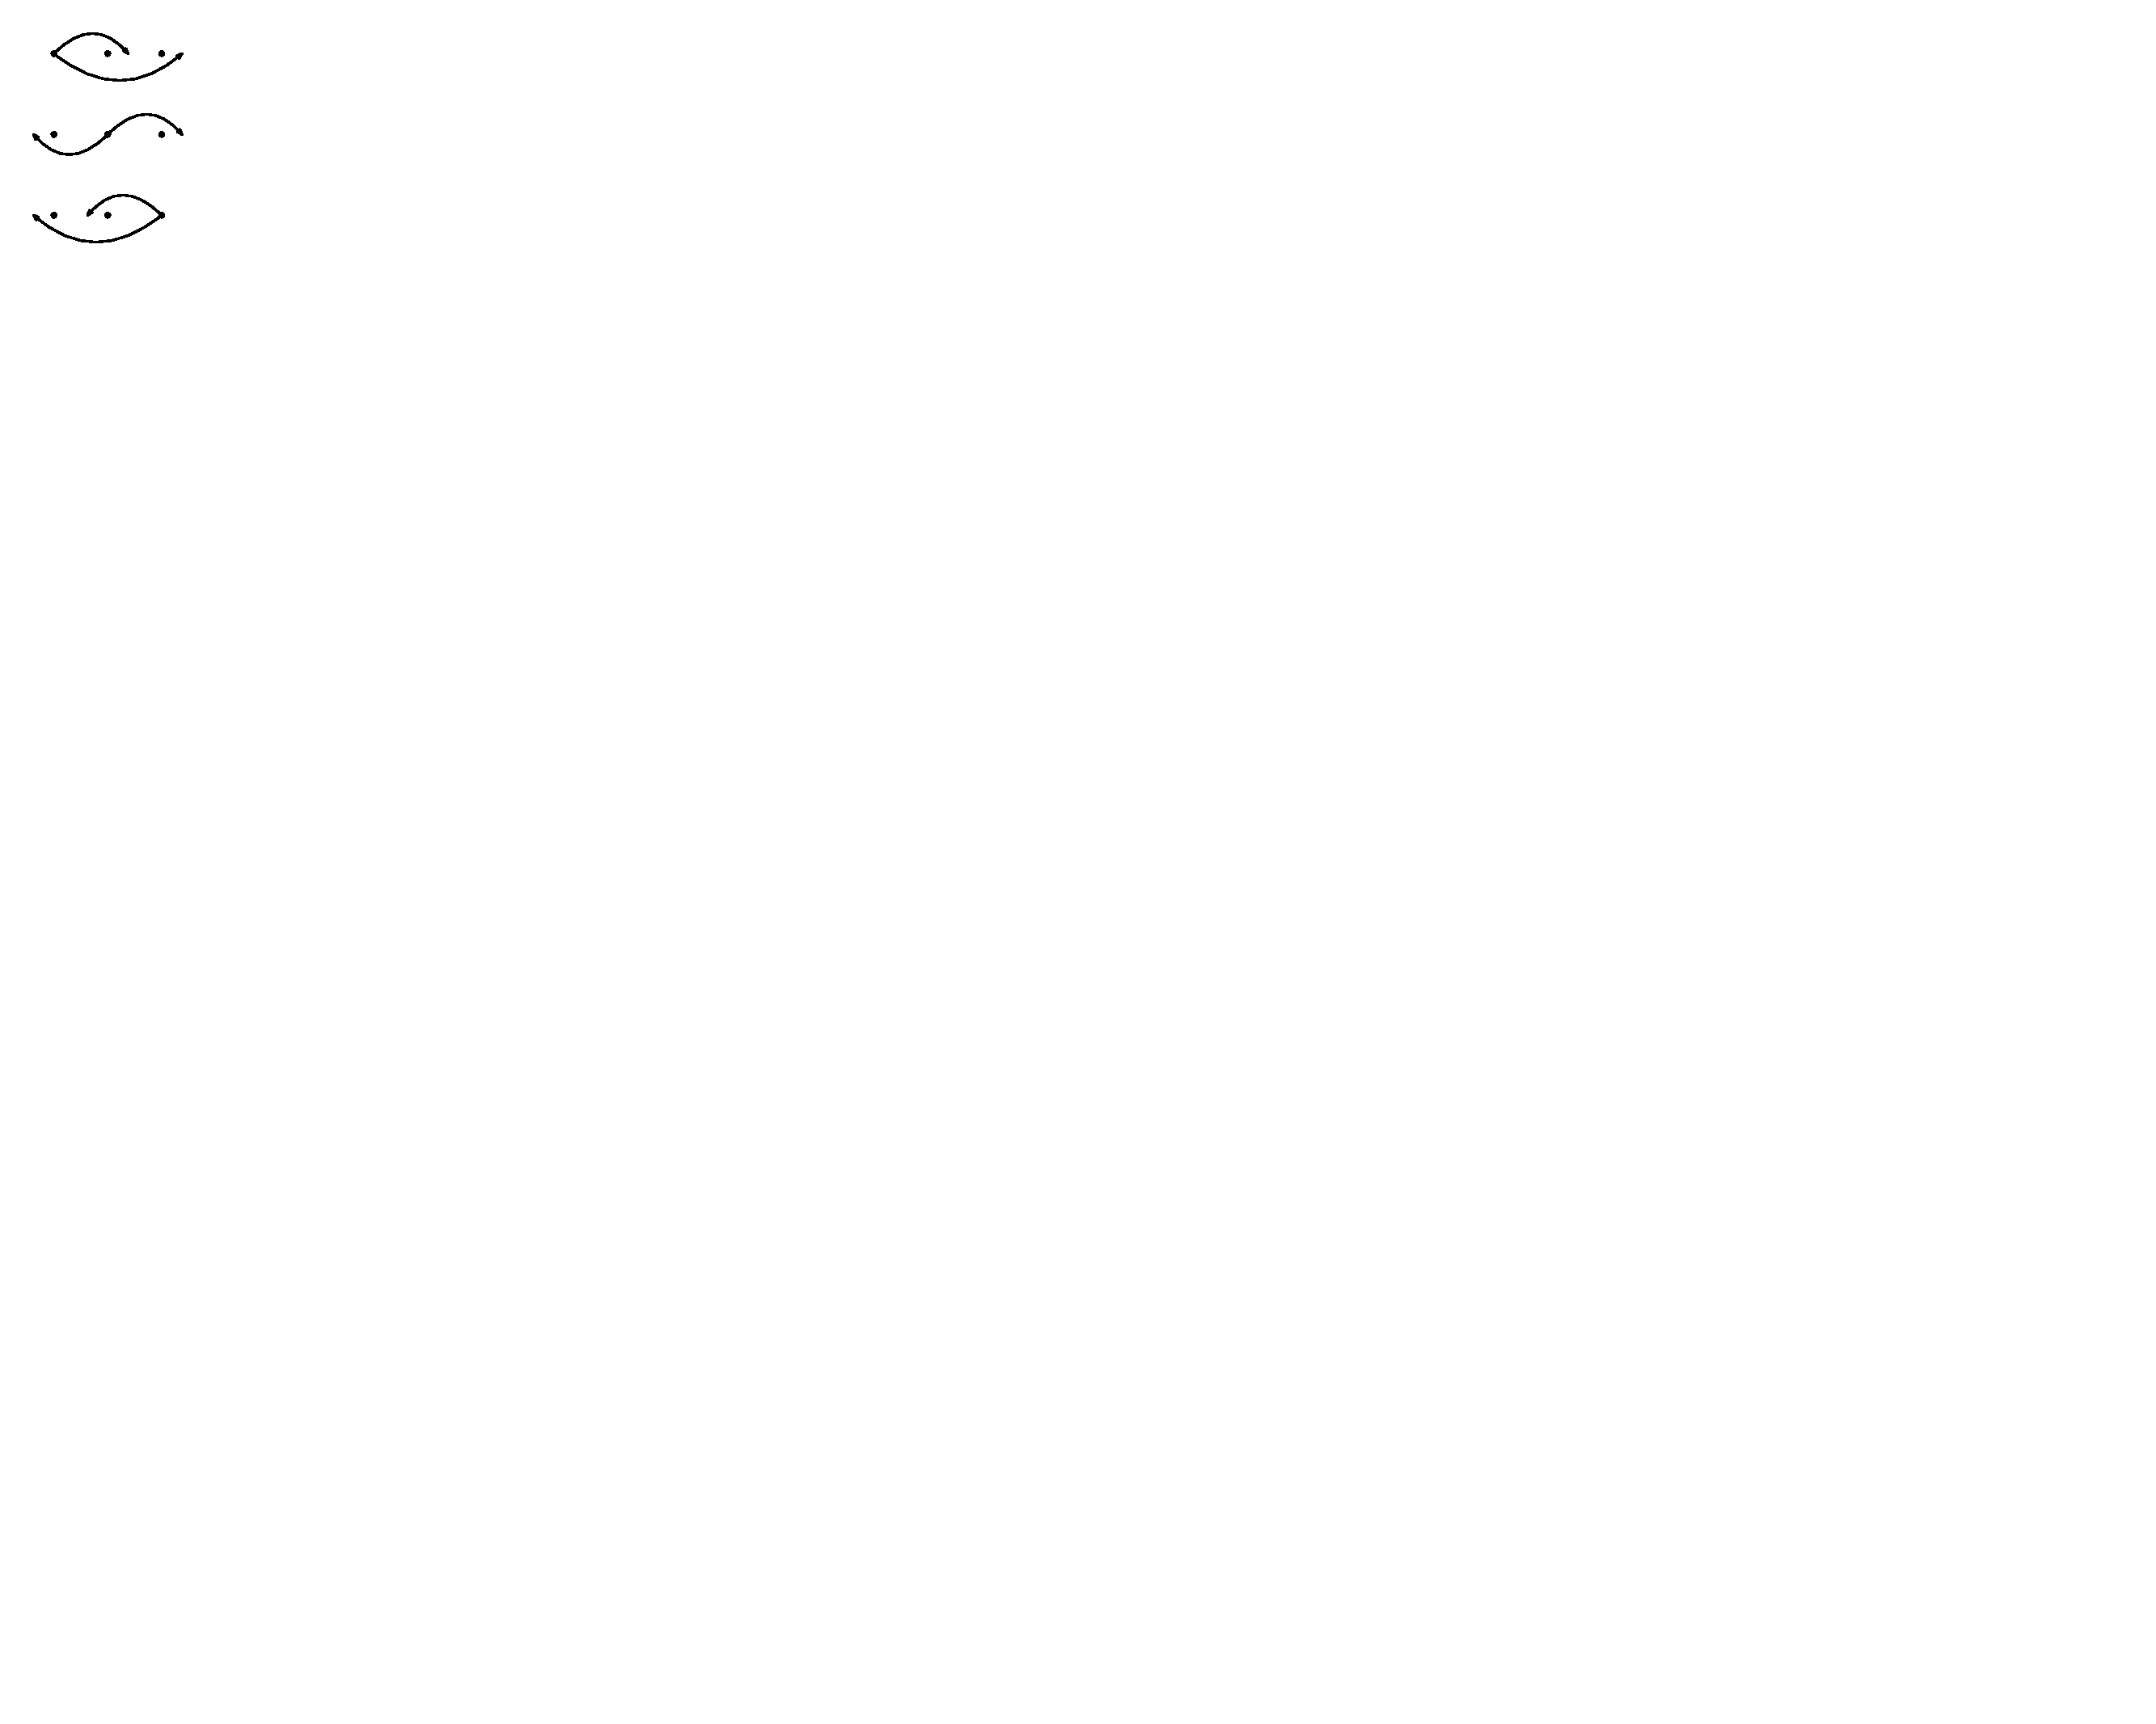
\includegraphics[scale=0.7]{figs/3_dots.pdf}
\caption{The six possible values the random variable $U_i$ can take when $n=3$.}
\label{3p}
\end{figure}
}

\subsection{The increase in contribution to SI}\label{sec-append-table}
We here illustrate in a table form the change in the contribution to SI at each
iteration. As can be seen there is a constant change in the contribution. The
table in Fig~\ref{fig-SI-contr-tab} summarized this finding.

\begin{figure}[h]
\begin{center}

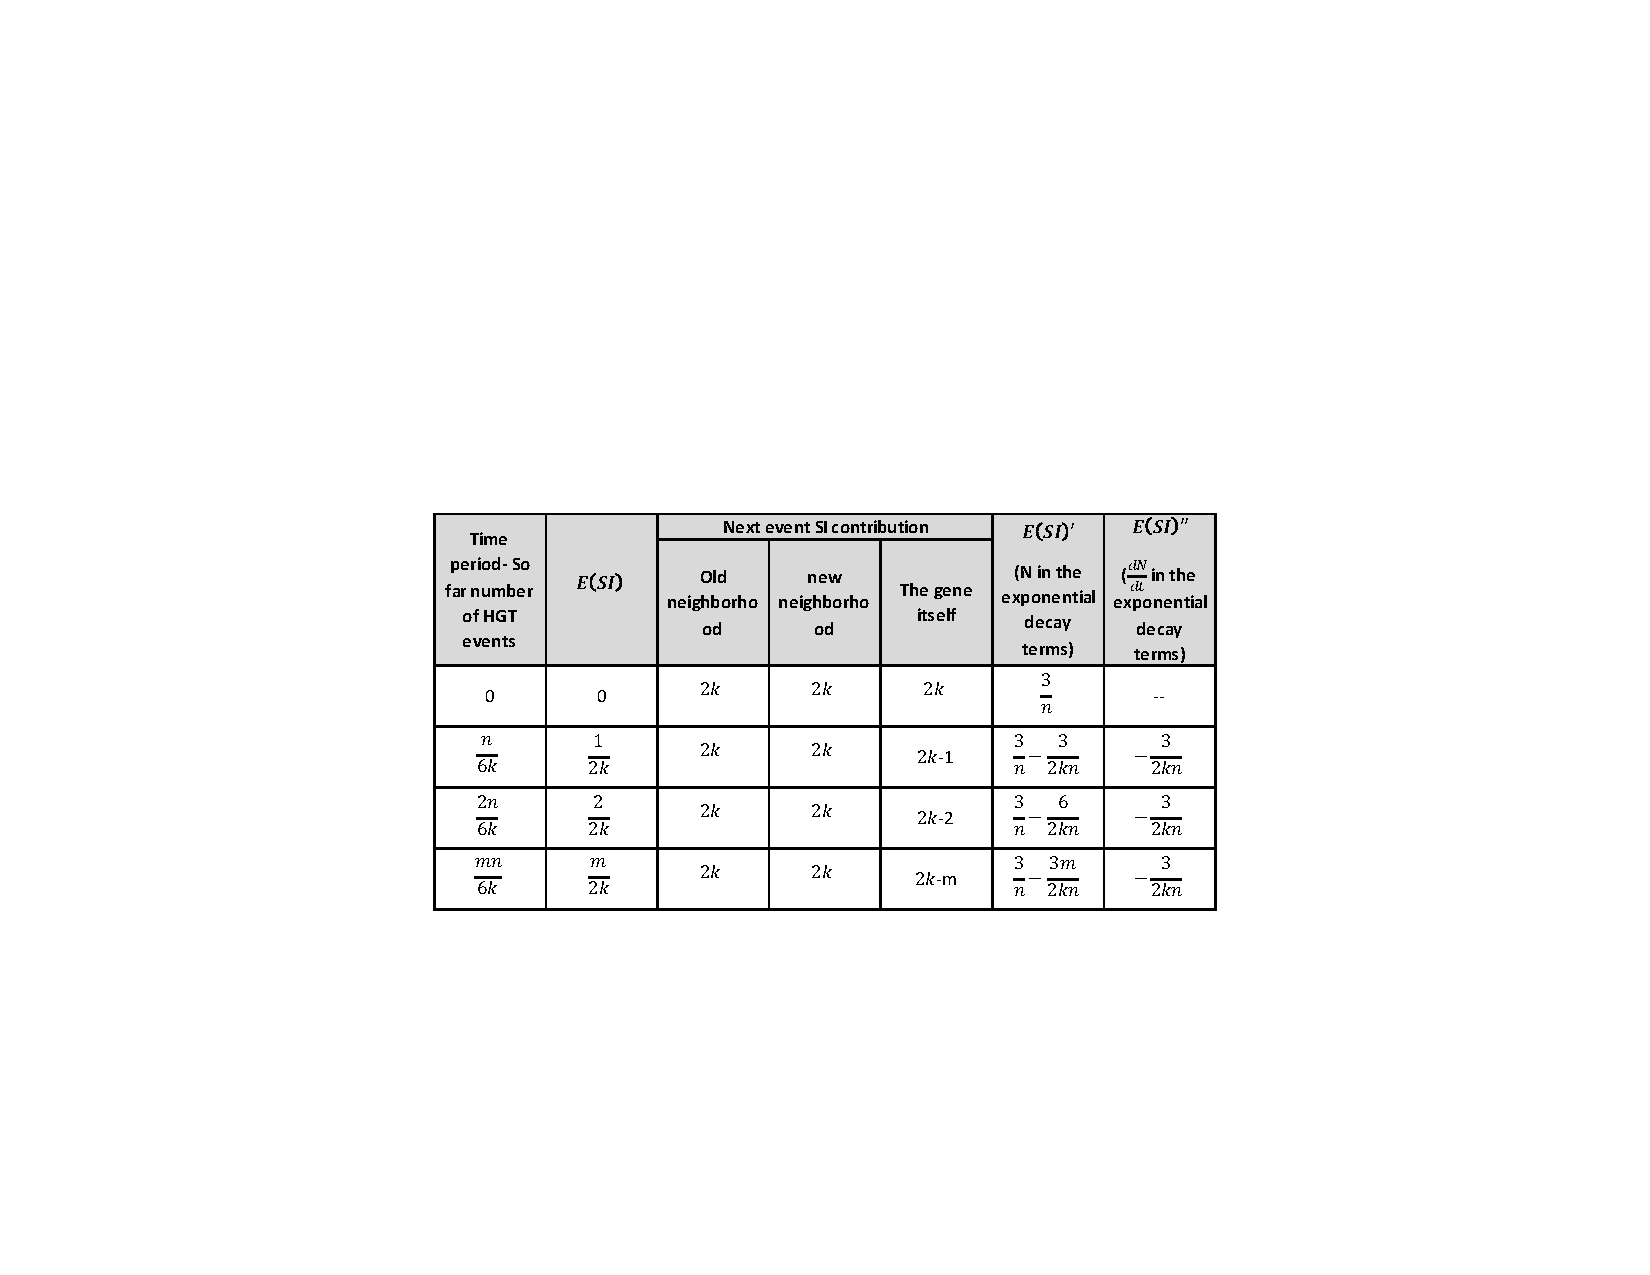
\includegraphics[width = 6in,angle=0]{figs/exp-decay-table.pdf} 
\caption{\small A manual calculation of the theoretical process for inferring
the instantaneous increase at the first three ``periods'' .
\label{fig-SI-contr-tab}}
 \end{center}
\end{figure}


\begin{figure}[h]
\vspace{-1in}
%\begin{center}
\hspace{-.9901cm}
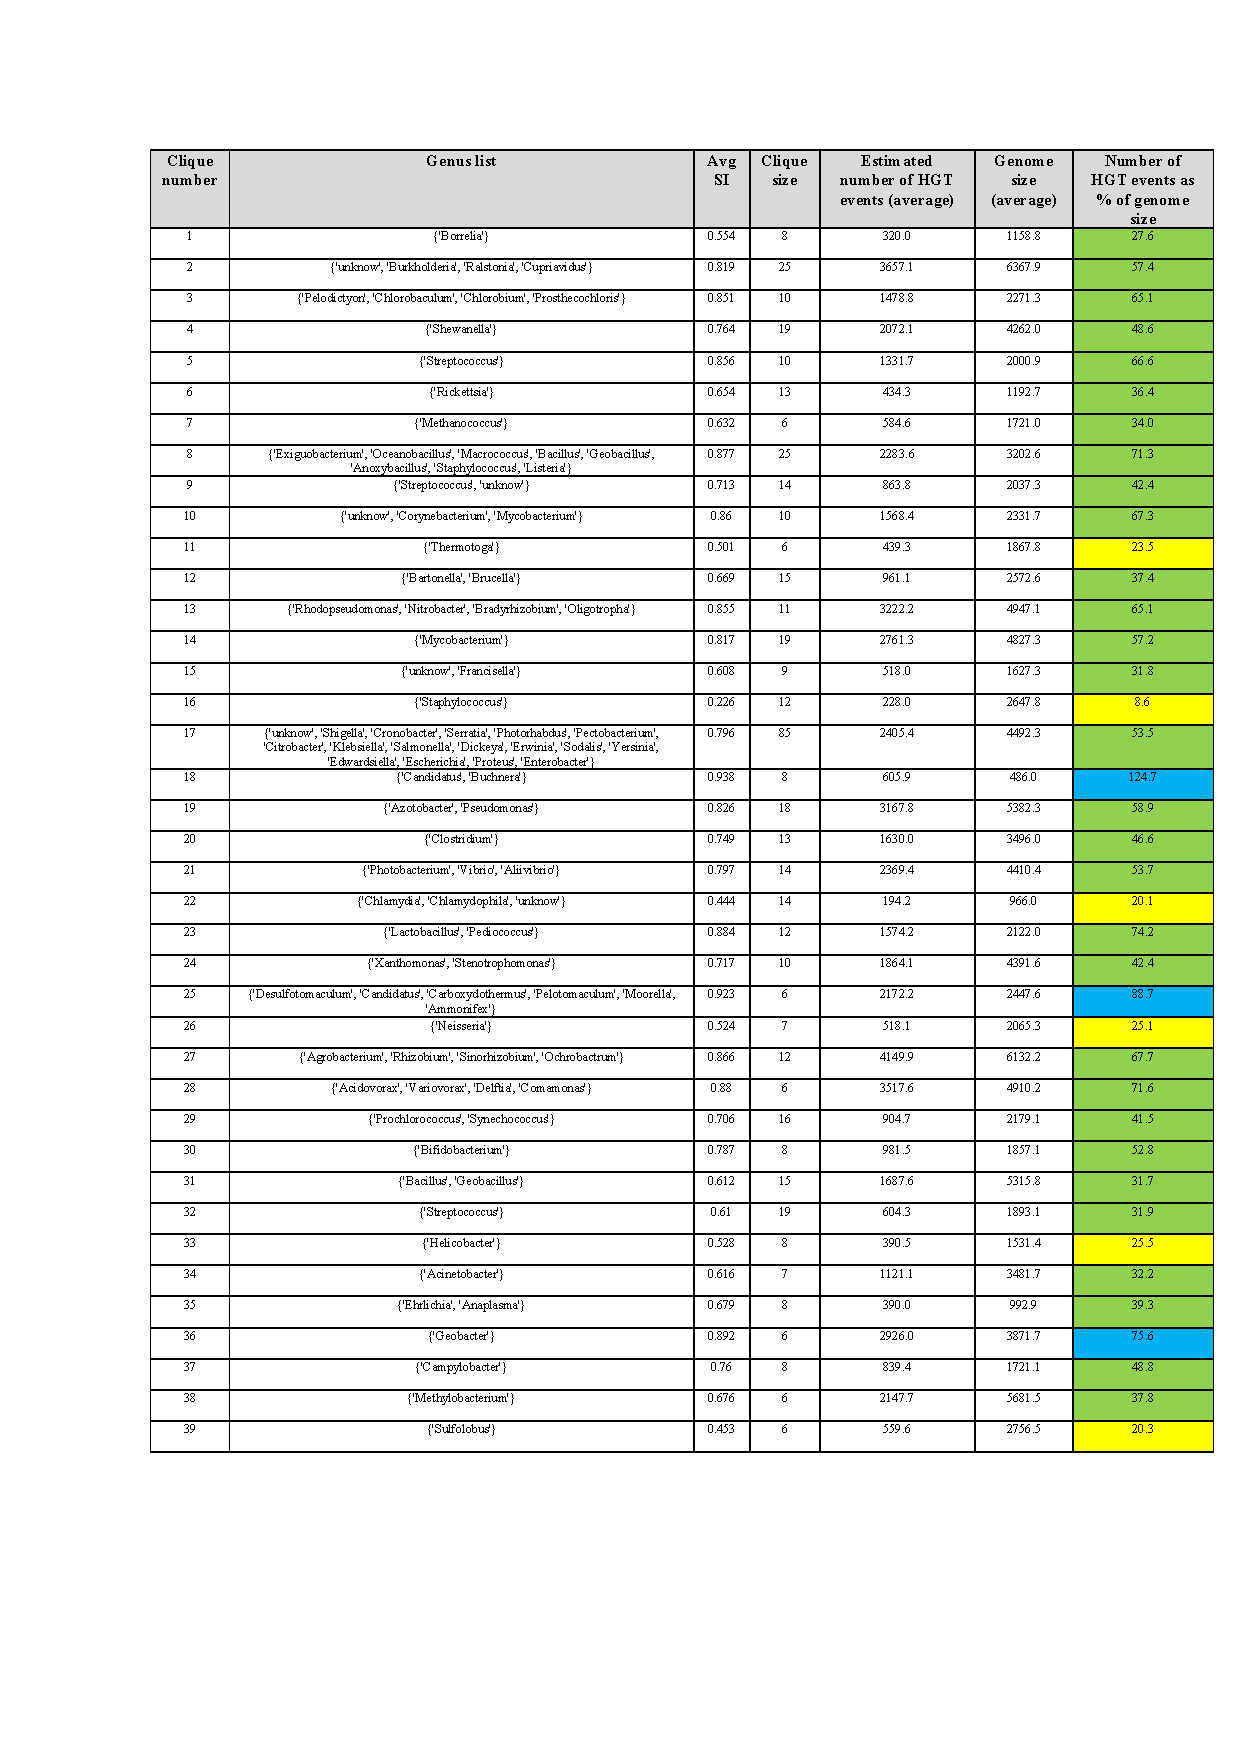
\includegraphics[scale=1,angle=0]{figs/real-data-table1.pdf} 
\caption{\small Real data results obtained for the 39 cliques derived by our
technique. For every clique, we reported the genus corresponding to it, the size
of the clique (\#genomes), average SI and its corresponding \#HGTs. The colors 
at the rightmost column signify distance fro average: In green- values fit the
range of 1SD from the mean (i.e., $>28.92$ and $<76.48$). In blue values higher
than 1SD from the mean ($\geq 76.48$). In yellow values lower more than 1SD from the
mean ($\leq 28.92$). \label{fig-real-data-table}}
\end{figure}


\end{document}
